%%%%%%%%%%%%%%%%%%%%%%%%%%%%%%%%%%%%%%%%%%%%%%%%%%%%%%%%%%%%%%%%%%%%%%%%%%%%%%%%%%%%%%%%%%%%%%%%%%%%
% ==================================================================================================
% --------------------------------------------------------------------------------------------------
\chapter{Experiment \& Results}\label{ch-exp}
Having defined each of the algorithm components, and derived the estimation procedures,
this section explores model validation and optimization.
Performance of model components is characterized with respect to intermediate objectives,
including graylevel standardization and regularization, in toy scenarios.
The segmentation performance of the full model is then presented
under several cross validation frameworks, and compared to a similar algorithm.
%%%%%%%%%%%%%%%%%%%%%%%%%%%%%%%%%%%%%%%%%%%%%%%%%%%%%%%%%%%%%%%%%%%%%%%%%%%%%%%%%%%%%%%%%%%%%%%%%%%%
\section{Data}\label{s:data}
For the several reasons (cf.~\ref{s:cv-frameworks})
it was important to collect a large and diverse database of FLAIR images for model validation.
Two datasets were defined using 129 FLAIR images from from 10 different scanners.
The number of images and scan parameters are summarized in Table~\ref{tab:database}.
Except for the MS 2008%
\footnote{The manual segmentations used in this dataset were generated in-house,
  as described in \S~\ref{ss:m08-rev}.}
and In-House datasets,
all of the data are freely available as part of the segmentation competitions.
Since direct comparison of results on equal datasets is important for establishing state-of-the-art,
results are primarily presented using only these freely available data (``Dataset A''),
though all the available data (``Dataset B'') are also used for some results.
The average distribution of WMH in Dataset A is shown in Figure~\ref{fig:mean-wmh} for reference.
\par
\begin{table}[t]
  % __JK__ please excuse this large table...
  \centering
  \caption{Summary of experimental image database.}%
  \label{tab:database}
  {\setlength{\tabcolsep}{4pt}
    \begin{tabu} to \textwidth {crclX[c]X[c]X[c]cc}
    	\toprule
    	Img  &                                      &                   &                    & TE   & TR    & TI   &         Voxel Size         & Manuals  \\
    	(\#) &                             Database &        Ref.       & Scanner            & (ms) & (ms)  & (ms) &            (mm)            &   (\#)   \\ \midrule
    	 20  & \sname{01} {\sclr{01}$\blacksquare$} & \cite{WMHSEG2017} & 3T Philips Achieva & 125  & 11000 & 2800 & $0.96\times0.96\times3.00$ & 1 \ss{a} \\ % chktex 2
    	 20  & \sname{02} {\sclr{02}$\blacksquare$} & \cite{WMHSEG2017} & 3T Siemens TrioTim & 82   & 9000  & 2500 & $1.00\times1.00\times3.00$ & 1 \ss{a} \\ % chktex 2
    	 20  & \sname{03} {\sclr{03}$\blacksquare$} & \cite{WMHSEG2017} & 3T GE Signa HDxt   & 126  & 8000  & 2340 & $0.98\times1.20\times3.00$ & 1 \ss{a} \\ % chktex 2
    	 5   & \sname{04} {\sclr{04}$\blacksquare$} & \cite{MSSEG2016}  & 3T Philips Ingenia & 360  & 5400  & 1800 & $0.50\times1.10\times0.50$ & 7 \ss{b} \\ % chktex 2
    	 5   & \sname{05} {\sclr{05}$\blacksquare$} & \cite{MSSEG2016}  & 1.5T Siemens Aera  & 336  & 5400  & 1800 & $1.04\times1.25\times1.04$ & 7 \ss{b} \\ % chktex 2
    	 5   & \sname{06} {\sclr{06}$\blacksquare$} & \cite{MSSEG2016}  & 3T Siemens Verio   & 399  & 5000  & 1800 & $0.74\times0.70\times0.74$ & 7 \ss{b} \\ % chktex 2
    	 21  & \sname{07} {\sclr{07}$\blacksquare$} & \cite{MSISBI2015} & 3T Philips         & 68   & 11000 & 2800 & $0.43\times0.43\times3.00$ & 2 \ss{c} \\ \midrule % chktex 2
    	 13  & \sname{08} {\sclr{08}$\blacksquare$} &       ---         & 3T Philips Achieva & 125  & 9000  & 2800 & $1.00\times1.00\times1.00$ & 1 \ss{d} \\ % chktex 2
    	 10  & \sname{09} {\sclr{09}$\blacksquare$} & \cite{MSSEG2008}  & ---                & ---  & ---   & ---  & $0.50\times0.50\times0.50$ & 1 \ss{e} \\ % chktex 2
    	 10  & \sname{10} {\sclr{10}$\blacksquare$} & \cite{MSSEG2008}  & 3T Siemens Allegra & 125  & 9000  & 2800 & $0.50\times0.50\times0.50$ & 1 \ss{f} \\ \bottomrule % chktex 2
    \end{tabu}}
  \tablepost{\ss{a}~Manuals were generated following the standards outlined in~\cite{Caligiuri2015},
    and were subsequently reviewed by a second rater, only WMH labels were included;
    \ss{b}~Manuals were fused using the LOP-STAPLE method~\cite{Akhondi-Asl2014};
    \ss{c}~Manuals were fused using logical `and';
    \ss{d}~Manuals were generated in-house;
    \ss{e}~[X];
    \ss{f}~[X].}
\end{table}
\begin{figure}
  \centering
  \includegraphics[height=\sliceheight]{mean-G.png}
  \includegraphics[height=\sliceheight]{cmap-mean-G}
  \caption{Average distribution of WMH in Dataset A. Best viewed in colour.}%
  \label{fig:mean-wmh}
\end{figure}
Regarding simulated MR images,
none are used for validation of segmentation performance in this work.
While such data (e.g.\ BrainWeb~\cite{Collins1998})
are useful for evaluation of whole-brain segmentation methods,
only three examples of WMH are currently available,
and there is little documentation as to how these were generated.%
\footnote{Documentation found here:
  \hreftt{http://brainweb.bic.mni.mcgill.ca/brainweb/selection_ms.html}.}
Furthermore, several works~\cite{Klauschen2009,Eggert2012} have noted significant discrepancies
in estimated segmentation performance between BrainWeb and real data (ISBR~\cite{IBSR}).
%%%%%%%%%%%%%%%%%%%%%%%%%%%%%%%%%%%%%%%%%%%%%%%%%%%%%%%%%%%%%%%%%%%%%%%%%%%%%%%%%%%%%%%%%%%%%%%%%%%%
\section{Segmentation Performance Metrics}\label{ss:exp-metrics}
Quantifying the performance of a model is essential to optimizing its design.
Typically, WMH segmentation performance is characterized in two respects:
voxel-wise agreement and total lesion load (LL) volume agreement.
When comparing the estimated class $\hat{c}$ to the ground truth class $c$,
each individual voxel can occupy one of four states (colours shown for future reference):
\begin{itemize}[itemsep=0pt,topsep=0pt]
  \item[\textcolor{green}{\scalebox{0.7}{$\blacksquare$}}]
  True Positive (TP):
  $c = 1$ and $\hat{c} = 1$,
  correctly predicted ``lesion''.
  \item[\textcolor{red}  {\scalebox{0.7}{$\blacksquare$}}]
  False Positive (FP):
  $c = 0$ and $\hat{c} = 1$,
  incorrectly predicted ``lesion''.
  \item[\textcolor{blue} {\scalebox{0.7}{$\blacksquare$}}]
  False Negative (FN):
  $c = 1$ and $\hat{c} = 0$,
  incorrectly predicted ``healthy''.
  \item[\textcolor{black}{\scalebox{0.7}{$\blacksquare$}}]
  True Negative (TN):
  $c = 0$ and $\hat{c} = 0$,
  correctly predicted ``healthy''.
\end{itemize}
Summing the number of voxels in each state over an entire image volume,
voxel-wise agreement can then be quantified using the following measures:
\begin{itemize}
  \item \textbf{Similarity Index (SI)}
  (\textsc{aka} Dice Similarity Coefficient, F1-Score)\\
  Measures overall segmentation performance:
  \begin{equation}
    SI = \dfrac{2TP}{2TP + FP + FN}.%
    \label{eq:si}
  \end{equation}
  \item \textbf{Precision (Pr)}
  (\textsc{aka} Overlap Fraction, Positive Predictive Value)\\
  Fraction of predicted predicted positives which are true positives:
  \begin{equation}
    Pr = \dfrac{TP}{TP+FP}.% % chktex 35
    \label{eq:pr}
  \end{equation}
  \item \textbf{Recall (Re)}
  (\textsc{aka} Sensitivity, True Positive Rate)\\
  Fraction of true positives which are predicted positive:
  \begin{equation}
    Re = \dfrac{TP}{TP+FN}.%
    \label{eq:re}
  \end{equation}
\end{itemize}
Each measure is $\in [0,1]$, where higher is better.
Note that typical performance metrics like accuracy and specificity are avoided,
since they include the $TN$ count in the numerator,
which is typically much larger than $TP + FP + FN$ combined -- i.e.\ $c=1$ is a rare event.
\par
Overall volume agreement between segmentations is characterized using
the 2-way mixed-effects single-rater absolute intraclass correlation coefficient (ICC)%
\footnote{Option \texttt{`A-1'} in the Matlab function \texttt{ICC} from
  \hreftt{https://www.mathworks.com/matlabcentral/fileexchange/22099}}%
~\cite{Koo2016}, while trends in over/undersegmentation with lesion load
are illustrated using Blant-Altman plots~\cite{Altman1983}.
%%%%%%%%%%%%%%%%%%%%%%%%%%%%%%%%%%%%%%%%%%%%%%%%%%%%%%%%%%%%%%%%%%%%%%%%%%%%%%%%%%%%%%%%%%%%%%%%%%%%
\section{Cross Validation Frameworks}\label{s:cv-frameworks}
Supervised segmentation models require the capacity to model
complex relationships between the input image(s) and output label images.
When models with large capacity are trained on
a dataset which does not represent the full gamut of potential input data,
they risk \textit{overfitting}: acquiring a bias towards the training data~\cite{Hawkins2004}.
The main problem associated with overfitting is decreased performance on new data
(\textsc{aka} generalization performance)~\cite{Hawkins2004}.
Popular techniques for characterizing this expected decrease include
cross validation (CV) procedures.
These involve splitting the $N$ available examples into training ($r$) and testing ($e$) subsets,
where the training data are used to fit the model parameters,
and the test data are used to approximate the expected generalization performance;
the data splits are usually repeated, randomly or exhaustively,
to ensure robust results~\cite{Arlot2010}.
The most popular CV frameworks include:
\begin{itemize}
  \item\textbf{LOO -- Leave-One-Out:}
  Use all images except one as the training set;
  use it as the test case ($N_r = N-1$; $N_e = 1$);
  repeat $N$ times.
  \\\textit{Benefit:} Close approximation of the expected generalization performance
  \\\textit{Drawback:} Expensive to compute -- $\mathcal{O}(N)$
  \item\textbf{KFCV -- K-Fold Cross Validation:}
  Use all images except a random batch of $B = N/K$ images as the training set;
  use these as the test set ($N_r = N-B$; $N_e = B$);
  repeat $K$ times (without replacement).
  \\\textit{Benefit:} Less expensive to compute -- $\mathcal{O}(N/K)$
  \\\textit{Drawback:} Worse approximation of the expected generalization performance
\end{itemize}
Many authors also validate their model using LOO-CV,
but only use images from a consistent source during training,
repeating the process for all sources.
%This only approximates performance on images from a consistent source,
%and therefore assumes that labelled training data
%will always be available from the use-case scanner.
This framework can be summarized as follows:
\begin{itemize}
  \item\textbf{OSAAT -- One-Scanner-At-A-Time:}
  Use all images from a single scanner ($N_s$) except one as the training set;
  use it as the test case ($N_r = N_s-1$; $N_e = 1$);
  repeat $N$ times.
  \\\textit{Benefit:} Estimates source-specific generalization performance
  \\\textit{Drawback:} Does not approximate generalization performance for new image sources
\end{itemize}
\par
It is worth noting one additional framework which
does not estimate model generalization performance,
but which lends insights into the capacity of the algorithm
to model the desired relationship.
This is actually to not use any cross validation at all:
\begin{itemize}
  \item\textbf{No CV -- No Cross Validation:}
  Train and test the model on all available data ($N_r = N_e = N$);
  no repetition.
  \\\textit{Benefit:} Characterize model limitations; least expensive to compute -- $\mathcal{O}(1)$
  \\\textit{Drawback:} Not a valid approximation of the expected generalization performance
\end{itemize}
These results can be seen as a cap on model performance
-- the estimated generalization performance should never exceed the performance under No-CV.
In models with high capacity, No-CV results would be expected near perfect,
due to obvious overfitting.
However, in models with stronger priors or imperfect assumptions,
No-CV results illustrate the best possible performance achievable
through optimization regularization components alone.
% ==================================================================================================
\subsection{Leave-One-Source-Out CV}
The choice of cross validation framework can have significant impacts
on the reported model performance (see~\cite{Arlot2010} for an in-depth review),
and there is at least one assumption of the above methods which is not always valid:
that examples are independent and identically distributed (iid).
This is not true for data originating from multiple sources with different underlying distributions
(e.g.\ MRI with different scan-parameter combinations)~\cite{Geras2013}.
In fact,~\citeauthor{Geras2013} show that in multi-source problems
where the expected use case involves data from entirely new sources,
random KFCV (and therefore also LOO, as a special case of KFCV with $B=1$)
significantly overestimates the generalization performance.
This is because random training fold selection allows the model
to perceive source-specific characteristics of the test examples,
which cannot be repeated for truly new examples.
In such scenarios, the author proposes the following:
\begin{itemize}
  \item\textbf{LOSO -- Leave-One-Source-Out:}%
  \footnote{The original name used by~\citeauthor{Geras2013} % chktex 42
    was ``Multi-Source Cross Validation''}
  Withhold all examples from source $s\in 1\dots S$ from the training set,
  and use these as the test set ($N_r$ = $N-N_s$; $N_e = N_s$);
  repeat $S$ times.
  \\\textit{Benefit:} Best approximation of the expected generalization performance
  in multi-source problems
  \\\textit{Drawback:} Still only an approximation
\end{itemize}
As noted in the introduction (cf.~\S~\ref{ss:priorlimits}),
there has been surprisingly limited use of data from multiple sources
for validation of WMH segmentation algorithms.
Moreover, CV frameworks vary widely among papers, and to the best of this author's knowledge,
no WMH algorithm has yet been validated using LOSO CV.
This represents a significant caveat to reported performances,
since MRI have many sources of variability (cf.~\S~\ref{ss:autochallenges}),
including scanner manufacturer, field strength, sequence parameters, resolution,
anatomical and disease variability.
As the aim of this work is to develop a segmentation algorithm
which will perform well on any given FLAIR MRI,
the LOSO framework was initially developed without knowledge of the work by~\citeauthor{Geras2013}.
However, this paper happily corroborates the importance of LOSO CV to the current work.
In this case, one data source is defined as a unique scanner-parameter combination.
% ==================================================================================================
%\subsection{Competition Frameworks}\label{ss:competitions}
%One notable exception to this trend in WMH algorithms have been
%segmentation competitions~\cite{MSSEG2008,MSISBI2015,MSSEG2016,WMHSEG2017}.
%These generally provide both multi-source datasets and a robust validation framework.
%Table~\ref{tab:datacomp}
%\begin{table}[h]
%  \centering
%  \caption{Summary of competition image databases.}%
%  \label{tab:datacomp}
%    \begin{tabu} to \textwidth {lccccc}
%      \toprule
%      && \multicolumn{2}{c}{Training} & \multicolumn{2}{c}{Testing} \\
%      Database     &       Ref.        & $I$ & $S$ & $I$ & $S$ \\ \midrule
%      WMH 2017     & \cite{WMHSEG2017} & 60  &  3  & 110 &  5  \\ % chktex 2
%      MS 2016      & \cite{MSSEG2016}  & 15  &  3  & 38  &  4  \\ % chktex 2
%      MS 2015 ISBI & \cite{MSISBI2015} & 21  &  1  & 61  &  1  \\ % chktex 2
%      MS 2008      & \cite{MSSEG2008}  & 20  &  2  & 32  &  2  \\ \bottomrule % chktex 2
%    \end{tabu}
%\end{table}
%\par\dots\par
%%%%%%%%%%%%%%%%%%%%%%%%%%%%%%%%%%%%%%%%%%%%%%%%%%%%%%%%%%%%%%%%%%%%%%%%%%%%%%%%%%%%%%%%%%%%%%%%%%%%
\section{Graylevel Standardization}\label{ss:exp-ystd-jsep}
The objective of graylevel standardization in this work is relatively simple:
voxel-wise separation of the lesion class from healthy tissues.
Two methods of quantifying this were proposed:
Equations (\ref{eq:zsep-diff}) and (\ref{eq:zsep-conv}).
Therefore, using these metrics,
the graylevel standardization techniques defined in \S~\ref{s:pre-ystd} were compared
for the FLAIR intensities in Dataset A, and only those voxels in the brain mask.
\par
Since the truly raw image intensities range from $[0,129]$ to $[0,77537]$,
some minimal standardization is required as a baseline and to allow visualization.
For this, range matching with $\bm{\epsilon} = [10^{-4},1-10^{-4}]$ is used.
Figure~\ref{fig:ystd-pmf-raw} illustrates the ``raw'' image PMFs from Dataset A
following this transformation.
Note that these PMFs differ appreciably from those simulated in Figure~\ref{fig:simflairplot},
particularly in the separation of tissue-distribution peaks.
This may be due to several of the challenges noted in \S~\ref{ss:autochallenges},
but overall highlights the difficulties of segmenting real versus simulated images.
\par
\begin{figure}
  \begin{subfigure}{0.495\textwidth}
    \centering
    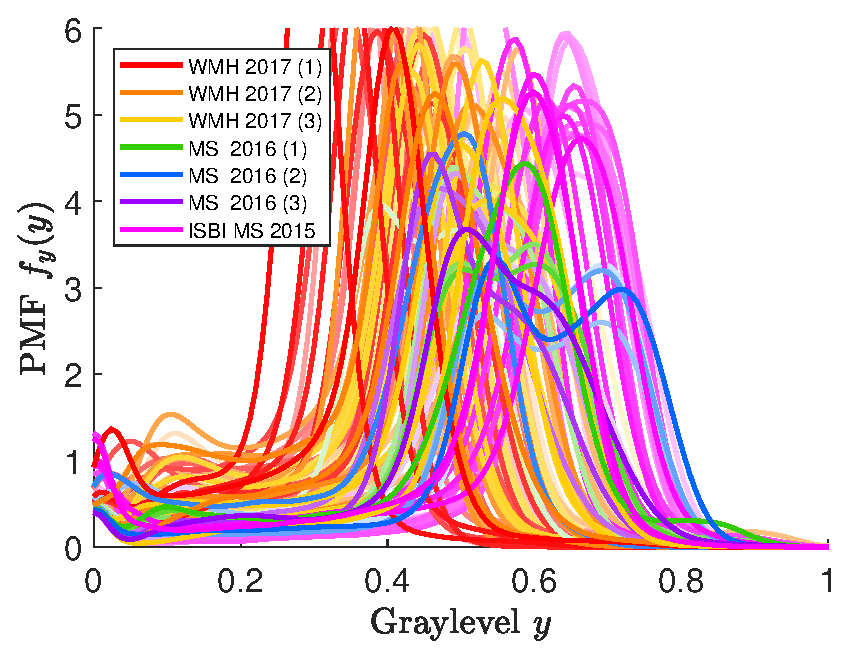
\includegraphics[width=\plotwidth]{ystd-pmf-na}
    \caption{Raw image PMFs before standardization.}%
    \label{fig:ystd-pmf-raw}
  \end{subfigure}
  \begin{subfigure}{0.495\textwidth}
    \centering
    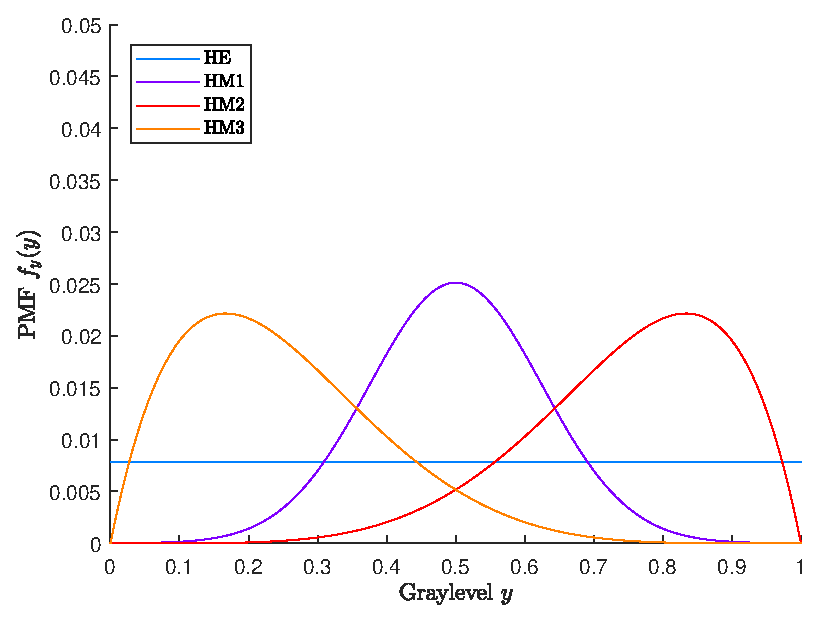
\includegraphics[width=\plotwidth]{ystd-pmf-hm123}
    \caption{Target PMFs for histogram matching operations.}%
    \label{fig:ystd-pmf-target}
  \end{subfigure}
  \caption{Image intensity PMFs. Best viewed in colour.}
\end{figure}
Next, each of the graylevel standardization techniques described in \S~\ref{s:pre-ystd}
were applied to the FLAIR intensity data.
For transforms with tunable parameters, several selections were made.
%as summarized in Table~\ref{tab:ystd-exp};
the target PMFs for histogram matching operations are also shown in Figure~\ref{fig:ystd-pmf-target}.
Both standardization objective functions were then computed for all voxels,
and averaged across the image.
Comparison of these metrics, shown in Table~\ref{tab:ystd-exp}, permits selection of the
best graylevel standardization technique.
\par
\begin{table}
  \centering
  \caption{Graylevel agreement objective functions (mean) for different standardization operations.}%
  \label{tab:ystd-exp}
  \begin{tabular}{llccl}
	\toprule
      $\uptau$ & Parameters & $\mathbb{E}[\Z_{\Delta}]$ & $\mathbb{E} [\Z_{\star}]$ & FFI\ss{a} \\ \midrule
	\textbf{RM1} & $\bm{\epsilon} = [10^{-4},1-10^{-4}]$           &   $16.1$    &   $7.42$    &         \\
	\textbf{RM2} & $\bm{\epsilon} = [10^{-3},1-10^{-3}]$           &   $16.7$    &   $7.70$    &         \\
	\textbf{RM3} & $\bm{\epsilon} = [10^{-2},1-10^{-2}]$           &   $15.5$    &   $7.52$    &         \\
	\textbf{SS}  & ---                                             &   $12.2$    & $\bm{5.77}$ & $\star$ \\
	\textbf{HE}  & ---                                             & $\bm{10.0}$ &   $8.16$    & $\star$ \\
	\textbf{HM1} & $f_{\tilde{y}} = \N(\frac{1}{2},\frac{1}{8})$   &   $11.5$    &   $6.86$    & $\star$ \\
	\textbf{HM2} & $f_{\tilde{y}} = \gamma^5-\gamma^6$             &   $12.0$    &   $9.11$    & $\star$ \\
	\textbf{HM3} & $f_{\tilde{y}} = {(1-\gamma)}^5-{(1-\gamma)}^6$ & $\bm{10.2}$ & $\bm{6.44}$ & $\star$ \\
	\textbf{NY}  & $Q = [0,\frac{1}{16},\dots,1]$                  &   $12.0$    &   $8.98$    &         \\ \bottomrule
\end{tabular}\\[0.5em]
\footnotesize{FFI: For further investigation.}
\end{table}
From these results, it can be seen that three transformations provide
good reductions in class graylevel overlap:
statistical standardization (\textbf{SS}),
histogram equalization (\textbf{HE}),
and the 3\ss{rd} histogram matching operation (\textbf{HM3}).
While the \textbf{HM3} operation is not optimal in either metric,
it achieved second place in both.
The worst results are given by
all three range-matching operations (\textbf{RM}),
the Nyul standardization method (\textbf{NY})
and the 2\ss{nd} histogram matching operation (\textbf{HM2});
therefore these will not be subject to further investigation.
\begin{figure}
  \centering
  \begin{subfigure}{\plotwidth}
    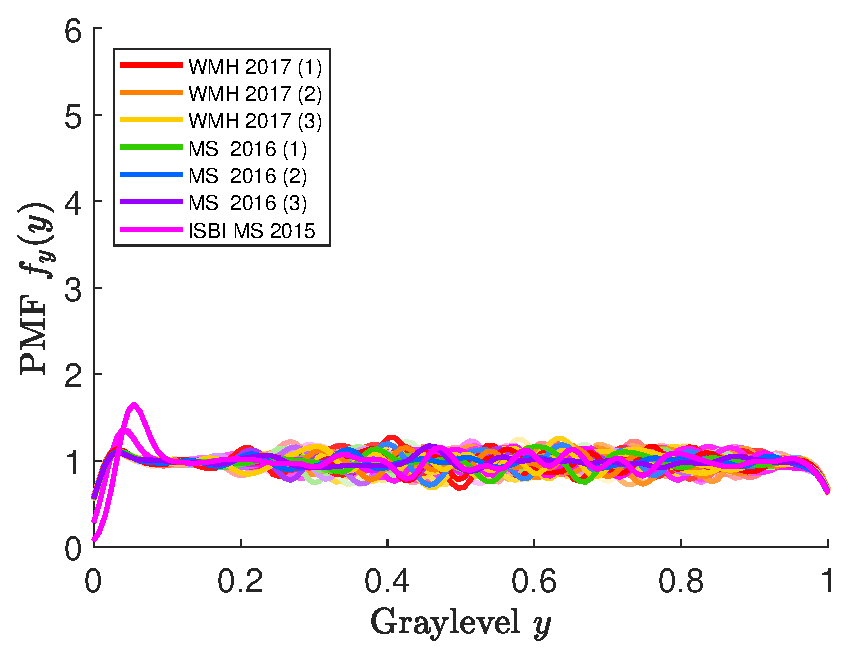
\includegraphics[width=\plotwidth]{ystd-pmf-he}
    \caption{Histogram Equalization (HE).}%
    \label{fig:ystd-pmf-he}
  \end{subfigure}
  \begin{subfigure}{\plotwidth}
    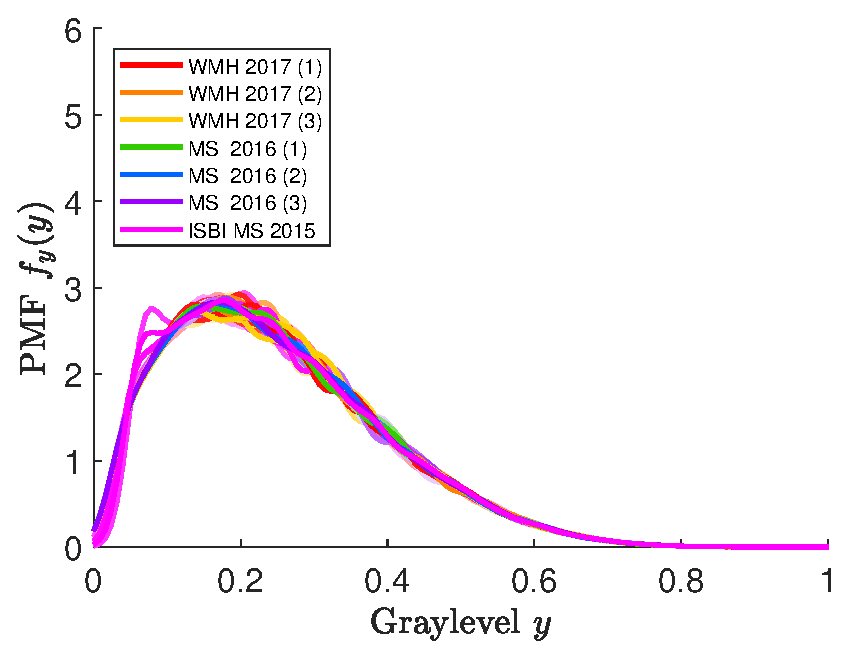
\includegraphics[width=\plotwidth]{ystd-pmf-m3}
    \caption{Histogram Matching 2: ``Left Skew'' (HM3).}%
    \label{fig:ystd-pmf-hm2}
  \end{subfigure}
  \caption{Image graylevel PMFs after the two best standardization operations.
    Best viewed in colour.}%
  \label{fig:ystd-pmf-best}
\end{figure}
Finally, since the graylevel agreement measures $Z_{\Delta}(x)$ and $Z_{\star}(x)$
are computed voxel-wise, it is possible to show their distribution spatially.
This is illustrated for the raw images and the best performing transformation:
\begin{figure}
 \subfigureoverl[white]{(a) $\Z_{\Delta}^{\textsc{raw}}(x)$}{}{%
      \includegraphics[height=\sliceheight]{ystd-zx-na-1.png}
      \includegraphics[height=\sliceheight]{cbar-zx-i-1}%
  }\\[0.5em]
  \subfigureoverl[white]{(b) $\Z_{\Delta}^{\textsc{hm}3}(x)$}{}{%
      \includegraphics[height=\sliceheight]{ystd-zx-op-1.png}
      \includegraphics[height=\sliceheight]{cbar-zx-i-1}%
  }\\[0.5em]
  \subfigureoverl[white]{(c) $\Z_{\Delta}^{\textsc{raw}}(x) - \Z_{\Delta}^{\textsc{hm}3}(x)$}{}{%
      \includegraphics[height=\sliceheight]{ystd-zx-naop-1.png}
      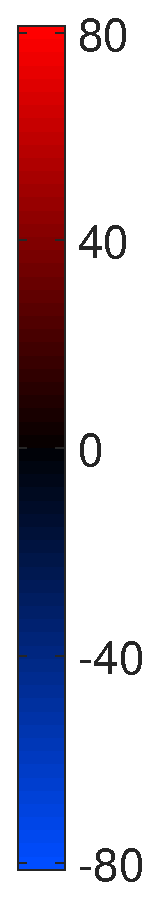
\includegraphics[height=\sliceheight]{cbar-zx-d-1}%
  }\\[0.5em]
  \subfigureoverl[white]{(d) $\Z_{\star}^{\textsc{raw}}(x)$}{}{%
    \includegraphics[height=\sliceheight]{ystd-zx-na-2.png}
    \includegraphics[height=\sliceheight]{cbar-zx-i-2}%
  }\\[0.5em]
  \subfigureoverl[white]{(e) $\Z_{\star}^{\textsc{hm}3}(x)$}{}{%
    \includegraphics[height=\sliceheight]{ystd-zx-op-2.png}
    \includegraphics[height=\sliceheight]{cbar-zx-i-2}%
  }\\[0.5em]
  \subfigureoverl[white]{(f) $\Z_{\star}^{\textsc{raw}}(x) - \Z_{\star}^{\textsc{hm}3}(x)$}{}{%
    \includegraphics[height=\sliceheight]{ystd-zx-naop-2.png}
    \includegraphics[height=\sliceheight]{cbar-zx-d-2}%
  }
  \caption{Spatial depiction of $\Z_{\Delta}(x)$ and $\Z_{\star}(x)$ comparing raw images 
    and images standardized using \textbf{HM3}.
  Best viewed in colour.}%
  \label{fig:jsep-diff-x-narm}
\end{figure}

\clearpage
%%%%%%%%%%%%%%%%%%%%%%%%%%%%%%%%%%%%%%%%%%%%%%%%%%%%%%%%%%%%%%%%%%%%%%%%%%%%%%%%%%%%%%%%%%%%%%%%%%%%
\section{Regularization}
This section explores the optimization of regularization strategies using a toy model,
in order to reduce the complexity of experimentation.
In particular,
the value of $\lambda$,
and the definition of pseudo-lesions $\{\bY_{\gamma},\bC_{\gamma}\}$
are explored, since these are implemented voxel-wise.
The segmentation performance of the full model under LOSO-CV
are later used to validate these results,
in addition to exploration of the other regularizations:
data augmentation and parameter image smoothing techniques.
% ==================================================================================================
\subsection{Toy Model}\label{ss:toy}
The toy model used here represents a single voxel during training, with synthetic observations.
Regularizations are then chosen to maintain desired characteristics in the fitted functions.
No specific objective function is defined for this purpose;
rather, the expected characteristics of the logistic function
illustrated in Figure~\ref{fig:chmle}
are used to empirically drive parameter selection.%
\footnote{This popular technique is also called ``hand waving''.}
In order to explore the various problem scenarios,
9 sets of synthetic data are generated
with the PMF shown in Table~\ref{tab:toy-pmf},
with the resulting distributions shown in Figure~\ref{fig:toy-data-pmf}.
\par
\begin{table}
  \centering
  \caption{Toy data definitions, with $y_c\sim\N(\mu_c,\sigma_c)$.}%
  \label{tab:toy-pmf}%
  \begin{tabular}{ccccccc}
\toprule
 & \multicolumn{3}{c}{$c=0$} & \multicolumn{3}{c}{$c=1$} \\
\cmidrule(lr){2-4}\cmidrule(lr){5-7}
\# & $\mu$ & $\sigma$ & $N$ & $\mu$ & $\sigma$ & $N$ \\
\midrule
a & 0.3 & 0.12 & 100 & 0.7 & 0.12 & 100 \\
b & 0.3 & 0.12 & 100 & 0.7 & 0.12 & 10 \\
c & 0.3 & 0.24 & 100 & 0.7 & 0.24 & 10 \\
d & 0.3 & 0.06 & 100 & 0.7 & 0.06 & 10 \\
e & 0.3 & 0.03 & 100 & 0.7 & 0.03 & 10 \\
f & 0.6 & 0.08 & 100 & 0.3 & 0.08 & 10 \\
g & 0.4 & 0.10 & 100 & --- & --- & 0 \\
h & 0.6 & 0.08 & 100 & --- & --- & 0 \\
i & 0.8 & 0.06 & 100 & --- & --- & 0 \\
\bottomrule
\end{tabular}
\end{table}
\begin{figure}
  \centering
  \foreach \i in {1,2,3,4,5,6,7,8,9}{% % chktex 1
    \begin{subfigure}{0.32\textwidth}
      \centering\includegraphics[width=\textwidth]{toy-pmf-\i}%
      \caption{}%
    \end{subfigure}\ }
  \caption{Synthetic data distributions (9 voxels) used in toy scenarios.}%
  \label{fig:toy-data-pmf}
\end{figure}
% ==================================================================================================
\subsection{Parameter Norm Penalties}\label{ss:exp-toy-lam}
Before exploring the 9 different scenarios specified above,
it is worth illustrating the effect of $L_2$ regularization
on the MAP objective function $\J(\bb)$ in the 2D plane composed of $\bb = [\b^0,\b^1]$.
Using synthetic dataset e, which would be expected to experience overfitting,
$\J(\bb)$ was computed over a grid of different $\b^0$ and $\b^1$ values.
The $\bb$ prior function $\P(\bb) = \norm{\bb}_2$ is computed similarly.
These functions are then exponentiated,
as in $J = e^{\J}$ and $P = e^{\P}$
-- i.e.\ the likelihood, as opposed to the log-likelihood.
For $\lambda = 0$,
the prior is a uniform distribution ($P(\bb) = 1$, Figure~\ref{fig:toy-srf-lamo}),
and the MAP objective equates the MLE objective ($J(\bb) = L(\bb)$, Figure~\ref{fig:toy-srf-lamy}).
For nonzero $\lambda = [10^{-3},10^{-2},10^{-1}]$, the MAP likelihood $J(\bb)$
can be defined as the product of $P(\bb\mid\lambda)$
(Figures~\ref{fig:toy-srf-lamo-3},~\ref{fig:toy-srf-lamo-2},~and~\ref{fig:toy-srf-lamo-1})
and $L(\bb)$ (Figure~\ref{fig:toy-srf-lamy}),
yielding Figures~\ref{fig:toy-srf-lamy-3},~\ref{fig:toy-srf-lamy-2},~and~\ref{fig:toy-srf-lamy-1}.
Thus, as expected, increasing $\lambda$ reduces the magnitudes of fitted $\bb$,
thereby limiting the slope parameter $s = \b^1$, as desired.
% __JK__ really this should only affect $\b^1$, and *not* $\b^0$
% (code is implemented this way)
% but this may add more confusion...
\par
\begin{figure}
  \centering
  \begin{subfigure}{0.32\textwidth}
    \centering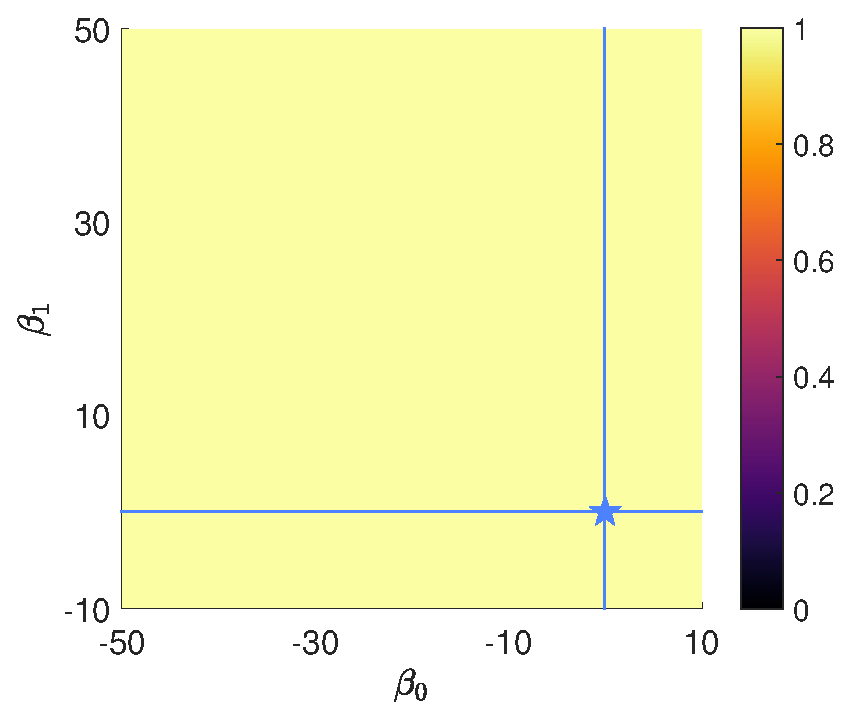
\includegraphics[width=\textwidth]{toy-srf-lamo-4}%
    \caption{$P(\bb) = 1,\quad\lambda = 0$}%
    \label{fig:toy-srf-lamo}
  \end{subfigure}
  \begin{subfigure}{0.32\textwidth}
    \centering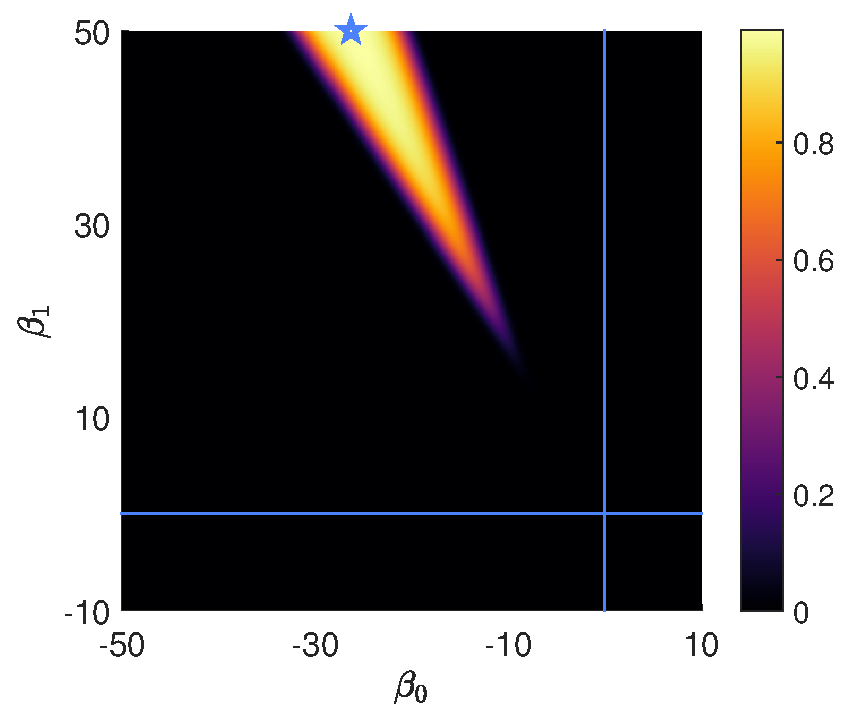
\includegraphics[width=\textwidth]{toy-srf-lamy-4}%
    \caption{$J(\bb) = L(\bb),\quad\lambda = 0$}%
    \label{fig:toy-srf-lamy}
  \end{subfigure}\\
  \foreach \i in {3,2,1}{% % chktex 1
    \begin{subfigure}{0.32\textwidth}
      \centering\includegraphics[width=\textwidth]{toy-srf-lamo-\i}%
      \caption{$P(\bb),\quad\lambda = 10^{-\i}$}%
      \label{fig:toy-srf-lamo-\i}
    \end{subfigure}
    \begin{subfigure}{0.32\textwidth}
      \centering\includegraphics[width=\textwidth]{toy-srf-lamy-\i}%
      \caption{$J(\bb),\quad\lambda = 10^{-\i}$}%
      \label{fig:toy-srf-lamy-\i}
    \end{subfigure}\\}
  \caption{Toy model likelihoods as a function of $\bb$:
    $P(\bb) = e^{\P(\bb)}$ and $J(\bb) = e^{\J(\bb)}$,
    for different $\lambda$, using scenario e.
    The optimum is shown as a blue star.
    Best viewed in colour.}%
  \label{fig:toy-srf-lam}
\end{figure}
\par
Next, the appropriate $\lambda$ is determined by
fitting the logistic model for the first 6 toy scenarios,
since the last 3 have no lesion class examples.
For each scenario, each of the same four $\lambda = [0,10^{-3},10^{-2},10^{-1}]$
are used to regularize the estimated parameters.
These results are shown in Figure~\ref{fig:toy-lam},
where the final state in each condition is shown in a different colour,
and the progression of the fitted logistic function is depicted from light to dark.
Note that a heuristic rule is used to ignore lesion observations
which are below the mean graylevel of the non-lesion class
-- i.e.\ the data $\{\Y_{c=1}\mid y<\mathbb{E}[\Y_{c=0}]\}$ are ignored;
this is demonstrated in scenario f.
%__JK__ this rule should be discussed elsewhere...?
\par
When the data from both classes overlap (scenarios a--c),
the results with and without regularization are roughly the same,
except for the strongest $\lambda = 10^{-1}$, which tends to have too much impact.
This implies that regularization in these scenarios is unnecessary,
and that the deviation from the MLE-fitted case ($\lambda = 0$) should be minimized,
so as to avoid biasing the model.
When the data from both classes do not overlap (scenarios d and e),
$\lambda$ plays an important role in limiting the magnitude of $\bb$.
Overall, $\lambda \in [10^{-3},10^{-2}]$ gives a good trade-off of
reduction in logistic slope in scenarios d and e,
and minimal impact in scenarios a--c.
\begin{figure}
  \centering
  \foreach \i in {1,2,3,4,5,6}{% % chktex 1
    \begin{subfigure}{0.32\textwidth}
      \centering\includegraphics[width=\textwidth]{toy-lam-\i}%
      \caption{}%
    \end{subfigure}\ }
  \caption{Toy model MAP estimation results for 6 different scenarios and different $\lambda$.
  Best viewed in colour.}%
  \label{fig:toy-lam}
\end{figure}
% ==================================================================================================
\subsection{Pseudo Lesion Regularization}\label{ss:exp-toy-psu}
Next, pseudo-lesion regularizations are explored,
namely selection of the number of synthetic lesions $V$.
Similar to above, only a subset of the scenarios are
originally problematic, and in need of this regularization;
these are the last four: f--i, where no typical lesions have been observed.
As before, the impact of the regularization should therefore
be minimal on the other scenarios, a--e.
Four selections of $V = [0,1,3,9]$ are used to train different models,
all with constant $\mathcal{V} = y_{\max} = 1$ and $\lambda = 10^{-3}$.
These results, presented in the same way as before, are shown in Figure~\ref{fig:toy-psu}.
\par
It can be seen that the inclusion of pseudo-lesions
has no appreciable impact on the first 5 scenarios, as desired.
In the problematic scenarios f--i,
the most significant change occurs with
the inclusion of the first pseudo-lesion ($V=0\rightarrow1$).
Larger values of $V$ have little impact,
but act to move $\tau$ slightly lower.
Therefore, the simple inclusion of one pseudo-lesion
may be all that is required.
Further investigations will explore this regularization with
segmentation performance results using the full model.
\par
\begin{figure}[h]
  \centering
  \foreach \i in {1,2,3,4,5,6,7,8,9}{% % chktex 1
    \begin{subfigure}{0.32\textwidth}
      \centering\includegraphics[width=\textwidth]{toy-psu-\i}%
      \caption{}%
    \end{subfigure}\ }
  \caption{Toy model MAP estimation results for 9 different scenarios and
    different numbers of pseudo-lesions $V$,
    shown as coloured diamonds corresponding to the scenario
    (spread of diamonds is for visualization only).
    Best viewed in colour.}%
  \label{fig:toy-psu}
\end{figure}
%%%%%%%%%%%%%%%%%%%%%%%%%%%%%%%%%%%%%%%%%%%%%%%%%%%%%%%%%%%%%%%%%%%%%%%%%%%%%%%%%%%%%%%%%%%%%%%%%%%%
\section{Full Modal -- Preliminaries}
Before exploring the segmentation performance of the full algorithm,
it is necessary to ensure that the model is converging during training,
and that the cross validation framework is appropriate.
It will also be helpful to establish a baseline model performance,
for comparison with model variants later.
These are the objectives of this section.
% ==================================================================================================
\subsection{Convergence}
The rate of convergence in each voxel will be unique.
During parallel fitting, it is prudent to stop training after
a maximum number of iterations, $t_{\max}$,
rather than wait for all voxels to achieve a certain stopping criterion,
in case a few aberrant voxels do not converge.
In order to determine this number, the model was fitted
using all available data from Dataset A, including augmentations
(reflection: $\mathrm{a}_{\textsc{r}} = \true$ and
shift one voxel in each dimension: $\mathrm{a}_{\textsc{s}} = \mathbf{N}_6$)
starting from the default initialization $\bb = {[0,0]}^T$ for all voxels.
The magnitude of $\Delta\beta$ (5\ss{th} to 95\ss{th} quantiles)
was recorded for each fitting iteration and plotted,
as shown in Figure~\ref{fig:converge}.
\par
\begin{figure}
  \centering
  \begin{subfigure}{\plotwidth}
    \centering
    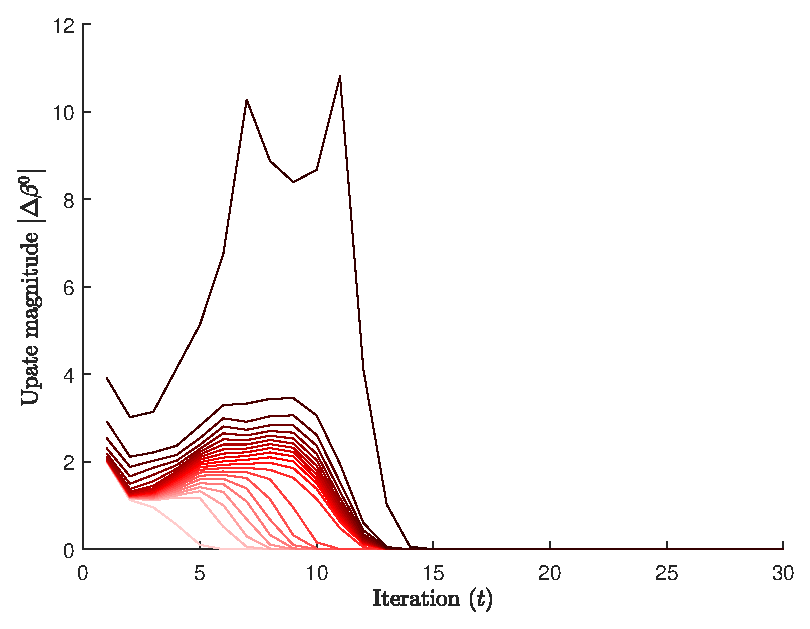
\includegraphics[width=\textwidth]{converge-b0}
    \caption{$\beta^0$}%
    \label{fig:converge-b0}
  \end{subfigure}
  \begin{subfigure}{\plotwidth}
    \centering
    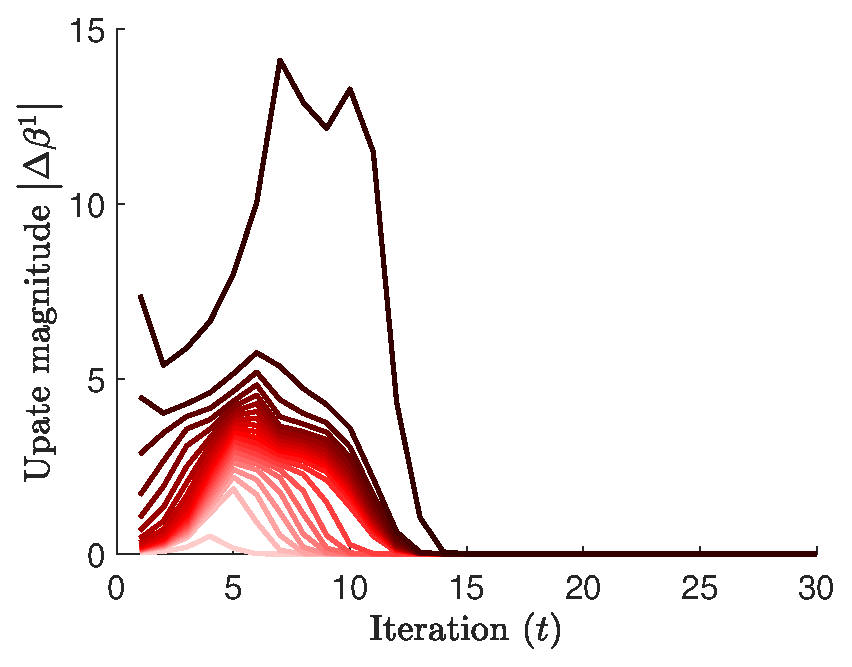
\includegraphics[width=\textwidth]{converge-b1}
    \caption{$\beta^1$}%
    \label{fig:converge-b1}
  \end{subfigure}
  \caption{Convergence characteristics of $\beta(x)$:
    quantiles ($0.00, 0.05, \dots, 1.00$) of the update magnitude $\left|\Delta\beta^{(t)}\right|$
    versus iteration $(t)$,
    using all augmented data.
    Convergence is apparent by the 15\ss{th} iteration.}%
  \label{fig:converge}
\end{figure}
Evidently, the majority of convergence occurs before the 15\ss{th} iteration.
Therefore, using a two-fold factor of safety, $t_{\max}$ was defined as 30
for all subsequent experiments.
% ==================================================================================================
\subsection{Cross Validation}\label{ss:exp-cv}
In \S~\ref{s:cv-frameworks}, it was argued that the LOSO-CV framework
gives a better estimation of generalization performance.
Practically speaking, this usually equates to a \textit{lower} estimated performance,
since the other CV frameworks described above allow perception of test scanner characteristics
within the training set, facilitating better performance.
In this section, the full model is trained and tested under each of the described CV frameworks,
in order to validate this assertion.
For a fair comparison with LOSO-CV, the KF-CV condition was implemented
using the same numbers of images in each fold.
Moreover, to avoid variance associated with random image selection,
the number of images assigned to each fold was guided by the expected value,
as illustrated in Figure~\ref{fig:bar-kfcv}.
The parameter selections for this version are summarized in Table~\ref{tab:hyp-final}.
Finally, it will be assumed that
the images have already been registered and transformed to MNI brain space
(cf.~\S~\ref{ss:spmdeform} for details about this workflow).
\par
\begin{figure}
  \centering
  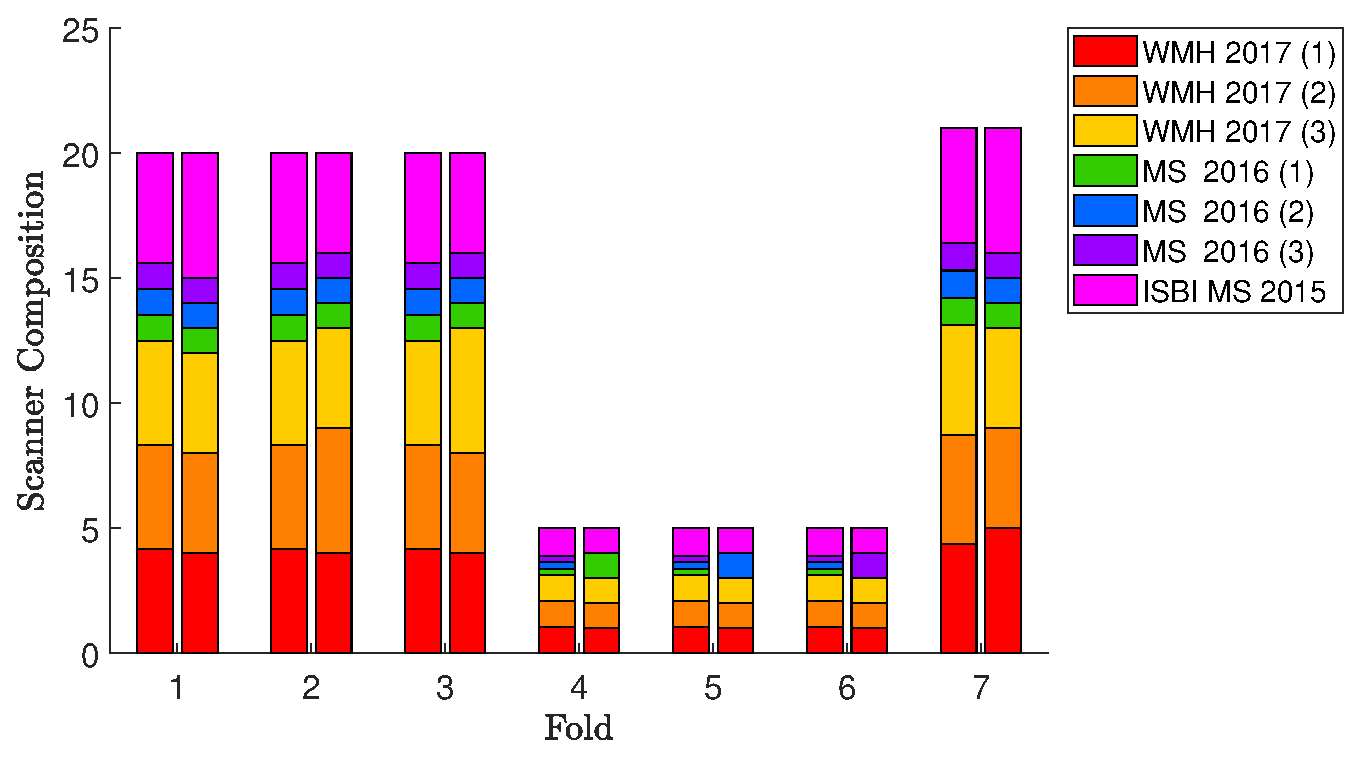
\includegraphics[width=1.5\plotwidth]{bar-kfcv}
  \caption{Number of images from each scanner in each KF-CV fold.
    Faded colours show the expected value (evenly distributed, non-whole numbers);
    full colours show the implementation (approximation, whole numbers).
    Best viewed in colour.}%
  \label{fig:bar-kfcv}
\end{figure}
The three performance metrics for each condition are
summarized using box plots in Figure~\ref{fig:seg-box-cv}.
The general trend in reported performance is as expected:
LOSO-CV $<$ KF-CV $\approx$ LOO-CV $\approx$ OSAAT-CV $<$ No-CV.
Ignoring the LL groupings (i.e.\ $N = 96$),
a paired non-parametric statistical test (\texttt{signrank} in MATLAB)
was used to test for significant differences among these conditions.
The No-CV condition reported significantly higher performance in both $SI$ and $Re$,
versus LOO-CV, KF-CV, and LOSO-CV, (6 of 6 comparisons).
This demonstrates the capacity of this model to overfit,
since training and testing on the same data yields better results
than any scenario where the test data are not seen during training.
The OSAAT condition gave consistently higher $Pr$, but lower $Re$ % chktex 35
versus all other conditions, yielding only significant differences in $SI$ with LOSO-CV.
This is most likely attributable to the smaller number of training examples,
since the training set in each fold comprises only same-scanner images.
\par
More importantly, the reported performance metrics
were significantly higher under LOO-CV and KF-CV than under LOSO-CV,
in all comparisons except $Re$ in LOO-CV vs LOSO-CV (5 of 6 comparisons).
This illustrates the potential overestimation of generalization performance
using classic CV techniques,
wherein scanner-specific characteristics of images in the test set
are perceived during training.
In reality, images from the use-case scanner are often not available for training,
so the proposed LOSO-CV framework should be used
to provide a better estimate of expected performance.
\par
\begin{figure}
  \centering
  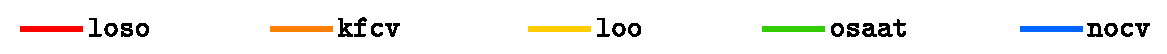
\includegraphics[scale=0.4]{cv-box-leg}\\[0.5em]
  \begin{subfigure}{0.32\textwidth}
    \centering\includegraphics[scale=0.4]{cv-box-si}
    \caption{$SI$}%
    \label{fig:seg-box-cv-si}
  \end{subfigure}
  \begin{subfigure}{0.32\textwidth}
    \centering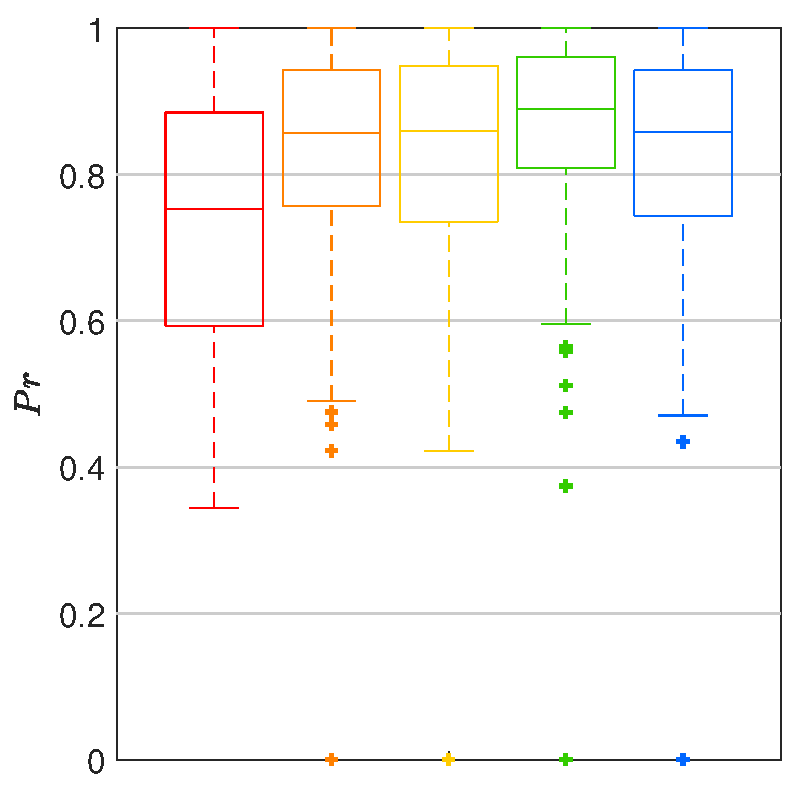
\includegraphics[scale=0.4]{cv-box-pr}
    \caption{$Pr$}% % chktex 35
    \label{fig:seg-box-cv-pr}
  \end{subfigure}
  \begin{subfigure}{0.32\textwidth}
    \centering\includegraphics[scale=0.4]{cv-box-re}
    \caption{$Re$}%
    \label{fig:seg-box-cv-re}
  \end{subfigure}
  \caption{Comparison of the estimated model performance
    using different cross validation methods.
    Box plots show
    median (centre line), 25\ss{th} and 75\ss{th} percentiles (box),
    extreme values (whiskers), and outliers ($+$).}%
  \label{fig:seg-box-cv}
\end{figure}
It is worth noting that the trend in differences
is most significant among Precision results (Figure~\ref{fig:seg-box-cv-pr}).
This implies that differences arise primarily from
the number of false positives (cf.~Equation (\ref{eq:pr})).
One explanation for this result is that each scanner has
a characteristic spatial distribution of hyperintense artifacts,
which can be ignored once it is perceived during training.
\par
In sum, these results support the discussion presented in \S~\ref{s:cv-frameworks},
which states that the LOSO-CV framework is the most challenging
cross validation paradigm, giving the most realistic estimate of
expected generalization performance on data from new scanners.
Therefore, this framework as used throughout the remaining analysis of segmentation performance.
% ==================================================================================================
\subsection{Baseline Model Performance}\label{ss:exp-base}
The next section will explore model variants which yield performance improvements;
therefore, results from a minimal working algorithm are first presented for sake of comparison.
The parameters of this version (``\texttt{base}'') is summarized in Table~\ref{tab:hyp-base}.
\par
The fitted parameter images from the baseline model
are shown in Figure~\ref{fig:beta-base}.
While the threshold image contains reasonable values (near $y_{\max}$)
in the regions typically containing WMH (Figure~\ref{fig:mean-wmh}),
there are obvious artifacts throughout both images,
corresponding to locations where no lesions were observed in the training set.
These voxels do not exhibit stable convergence properties without regularization,
hence necessity of a static $t_{\max}$.
Classification results in any of these voxels will almost certainly be wrong;
therefore, overcoming these artifacts is a priority
during investigation of regularization strategies.
\par
\begin{figure}
  \centering
  \subfigureoverl[white]{$\mathcal{T}(x)$}{}{%
    \includegraphics[height=\sliceheight]{base-T.png}
    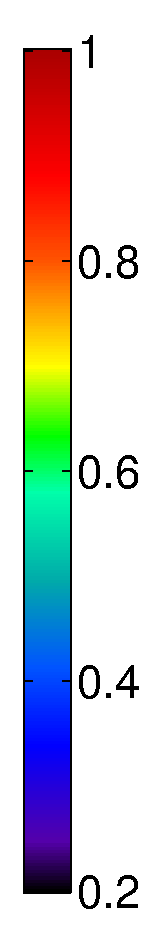
\includegraphics[height=\sliceheight]{base-cmap-T}}\\[0.5em]
  \subfigureoverl[white]{$\mathcal{S}(x)$}{}{%
    \includegraphics[height=\sliceheight]{base-S.png}
    \includegraphics[height=\sliceheight]{base-cmap-S}}
  \caption{Fitted parameter images $\mathcal{T}(x)$ and $\mathcal{S}(x)$
    from the first LOSO-CV fold of the baseline model.
    Obvious artifacts arise from inadequate regularization.
    Best viewed in colour.}%
  \label{fig:beta-base}
\end{figure}
After training and testing this version of the model under LOSO-CV,
the median performance metrics are summarized in Table~\ref{tab:seg-base};
the same metrics are illustrated in Figure~\ref{fig:seg-base}, stratified by LL tertiles.
The overall median SI was 0.63, Precision 0.77, and Recall 0.63.
Considering the artifacts in Figure~\ref{fig:beta-base},
these results are surprisingly good,
rivalling many of the reported performances in Table~\ref{tab:priorworkval},
which were obtained using much less challenging validation conditions.
As is often the case, performance is correlated with LL,
since voxel misclassifications have a larger effect
when the number of positive examples is small.
\par
With $Pr > Re$, it can be inferred that % chktex 35
the model incurs more FN than FP -- i.e.\ it is more specific than sensitive.
This would therefore predict an underestimation of the total LL.
The performance among the three MS 2016 scanners is also low.
This may be attributable to their notably different TE/TR/TI parameters
(Table~\ref{tab:database}), which are simulated in Figure~\ref{fig:simflair}.
In particular, a large performance drop is observed for
the data from Scanner 2 in the MS 2016 dataset;
two factors may help explain these results.
First, this is the only 1.5T scanner in the dataset,
which implies higher levels of noise due to
smaller MR signal magnitude during image acquisition.
Second, the median LL for these subjects was only 5 mL,
which is expected to correlate with decreased performance, as noted above.
\par
\begin{table}
  \centering
  \caption{Baseline model performance metrics (median)}%
  \label{tab:seg-base}
  \begin{tabular}{rcccc}
\toprule
Scanner & LL & SI & Pr & Re \\
\midrule
WMH 2017 (1) {\color[rgb]{ 1.00 0.00 0.00}$\blacksquare$} & 24 & 0.66 & 0.75 & 0.68 \\
WMH 2017 (2) {\color[rgb]{ 1.00 0.50 0.00}$\blacksquare$} & 17 & 0.77 & 0.78 & 0.73 \\
WMH 2017 (3) {\color[rgb]{ 1.00 0.80 0.00}$\blacksquare$} & 6 & 0.67 & 0.67 & 0.77 \\
MS  2016 (1) {\color[rgb]{ 0.20 0.80 0.00}$\blacksquare$} & 29 & 0.49 & 0.86 & 0.50 \\
MS  2016 (2) {\color[rgb]{ 0.00 0.40 1.00}$\blacksquare$} & 5 & 0.38 & 0.51 & 0.32 \\
MS  2016 (3) {\color[rgb]{ 0.60 0.00 1.00}$\blacksquare$} & 10 & 0.61 & 0.74 & 0.50 \\
ISBI MS 2015 {\color[rgb]{ 1.00 0.00 1.00}$\blacksquare$} & 5 & 0.62 & 0.58 & 0.76 \\
\midrule
ALL {\color[rgb]{ 1.00 1.00 1.00}$\blacksquare$} & 12 & 0.64 & 0.70 & 0.70 \\
\bottomrule
\end{tabular}
\end{table}
\begin{figure}
  \centering
  \begin{subfigure}{0.32\textwidth}
    \centering
    \includegraphics[width=\textwidth]{base-box-si}
    \caption{Similarity Index (SI)}%
    \label{fig:seg-base-si}
  \end{subfigure}
  \begin{subfigure}{0.32\textwidth}
    \centering
    \includegraphics[width=\textwidth]{base-box-pr}
    \caption{Precision (Pr)}%
    \label{fig:seg-base-pr}
  \end{subfigure}
  \begin{subfigure}{0.32\textwidth}
    \centering
    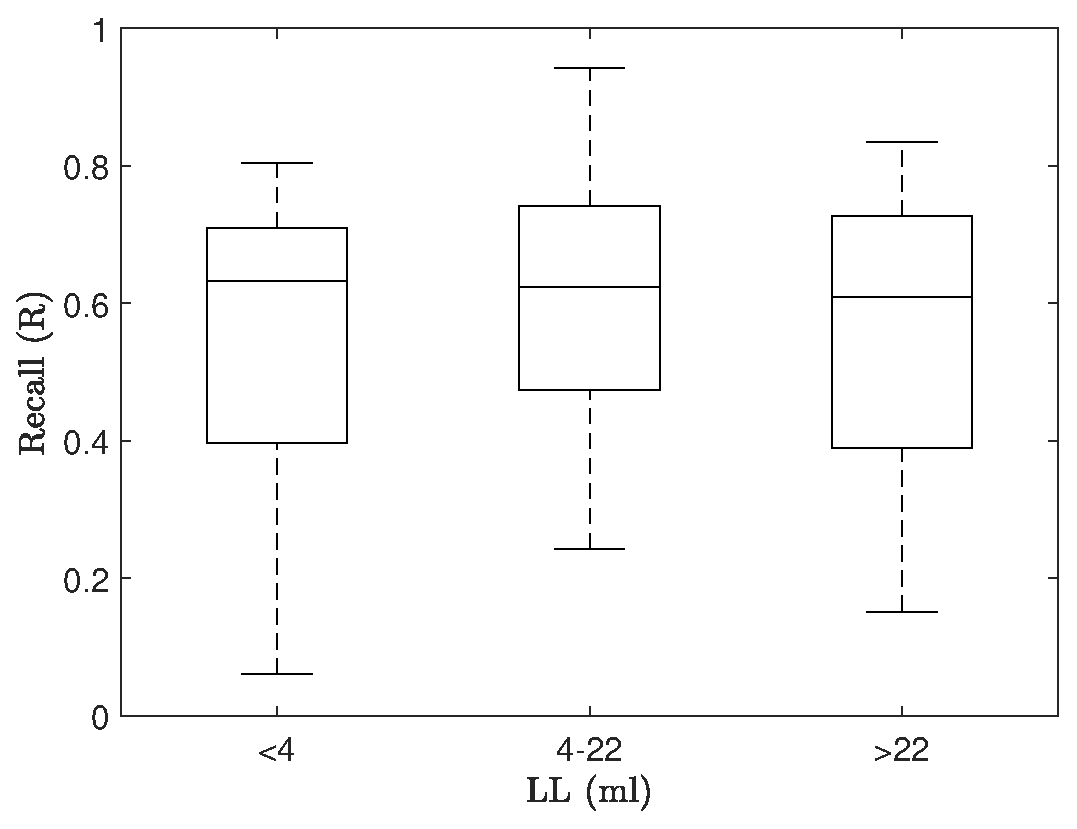
\includegraphics[width=\textwidth]{base-box-re}
    \caption{Recall (Re)}%
    \label{fig:seg-base-re}
  \end{subfigure}
  \caption{Baseline model performance, stratified by LL tertiles.}%
  \label{fig:seg-base}
\end{figure}
%Figure~\ref{fig:ba-base} shows the volume agreement between
%the manually segmented WMH and the VLR-predicted WMH.
%As predicted by the $Pr$ and $Re$ results,
%the model tends to underestimate the LL,
%with underestimation getting worse for very high LL.
%Correction of this error will be one aim of the parameter exploration in the next section.
%\par
%\begin{figure}
%  \centering
%  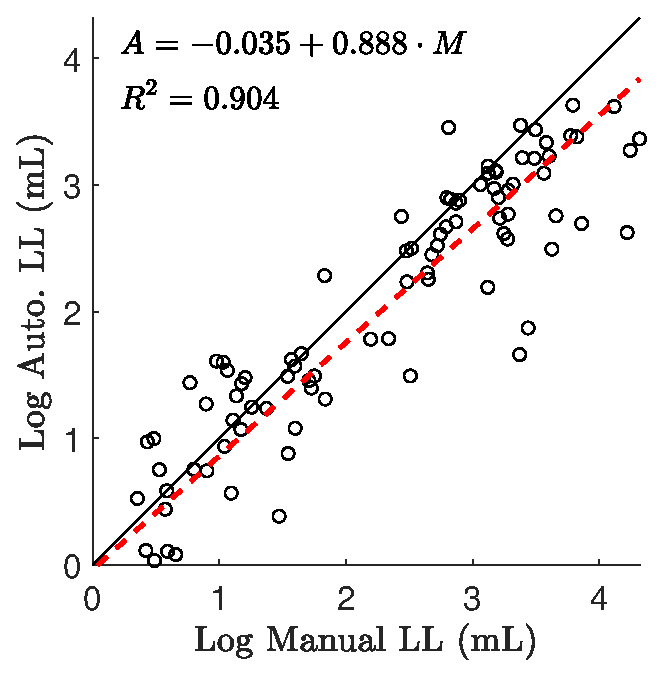
\includegraphics[width=\plotwidth]{base-ba-1}
%  \includegraphics[width=\plotwidth]{base-ba-2}
%  \caption{Bland-Altman plot showing total LL agreement between manual and VLR-segmented WMH.
%    Shown in Log-scale to better illustrate results for small LL.}%
%  \label{fig:ba-base}
%\end{figure}
%%%%%%%%%%%%%%%%%%%%%%%%%%%%%%%%%%%%%%%%%%%%%%%%%%%%%%%%%%%%%%%%%%%%%%%%%%%%%%%%%%%%%%%%%%%%%%%%%%%%
\section{Full Model -- Performance Results}
Next, the full model is trained and tested under a large variety of different conditions.
The results above are validated in terms of segmentation performance,
and optimization of additional model components is explored similarly.
Except where specified, the model will be trained and tested
as per the LOSO-CV framework, using Dataset A.
Additionally, while the above performance measures serve as a baseline,
an optimal combination of parameters was eventually resolved;
these parameters are summarized in Table~\ref{tab:hyp-final}, \S~\ref{ss:hyp-final}.
In many cases, the optimized parameters are essential for good model performance,
so these are used during exploration of other model components.
This parametrization is denoted ``\texttt{default}'', when compared against other model variants.
% ==================================================================================================
\subsection{Graylevel Standardization}\label{ss:exp-ystd-seg}
Five graylevel standardization techniques with promising results
predicted by the objective functions were
identified in \S~\ref{ss:exp-ystd-jsep} (cf.~Table~\ref{tab:ystd-exp}).
Each of these methods was applied to Dataset A,
yielding the contrast characteristics shown in Figure~\ref{fig:ystd-y}.
Next, the VLR model was trained and tested using these data,
and the segmentation performance results were compared.
Figure~\ref{fig:seg-box-ystd} compares the results under each condition,
again using box plots stratified by LL tertiles.
\par
\begin{figure}
  \centering
  \foreach \s/\cap in {% % chktex 1
    ss/$SS$,%
    he/$HE$,%
    m1/$HM1$,%
    m2/$HM2$,%
    m3/$HM3$}{%
    \subfigureoverl[white]{\cap}{}{%
      \includegraphics[height=\sliceheight]{ystd-\s-Y.png}
      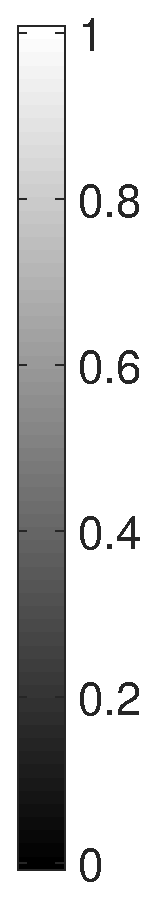
\includegraphics[height=\sliceheight]{cmap-ystd}
    }\\[0.5em]}
  \caption{Simulated FLAIR images after graylevel standardization
    using each technique under investigation.}%
  \label{fig:ystd-y}
\end{figure}
While statistical standardization (\textbf{SS})
outperforms all other techniques for subjects with high LL,
limitations in $Re$ at low and medium LL resulted in worse performance overall.
Histogram equalization (\textbf{HE}) was similarly afflicted by poor $Pr$ % chktex 35
at low and medium LL, yielding suboptimal $SI$ performance.
Two histogram matching operations, (\textbf{HM1} and \textbf{HM3})
having higher contrast at the upper end of the graylevel range,
were more successful in terms of segmentation performance.
Considering the near equivalence of these two methods (paired $SI$ test: $p = 0.4923$),
the objective function results from \S~\ref{ss:exp-ystd-jsep}
were used to select \textbf{HM3} as the optimal method going forward.
\par
\begin{figure}
  \centering
  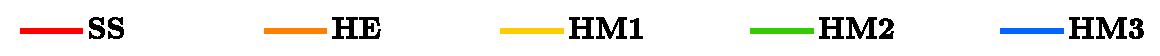
\includegraphics[scale=0.4]{ystd-box-leg}
  \begin{subfigure}{0.9\textwidth}
    \centering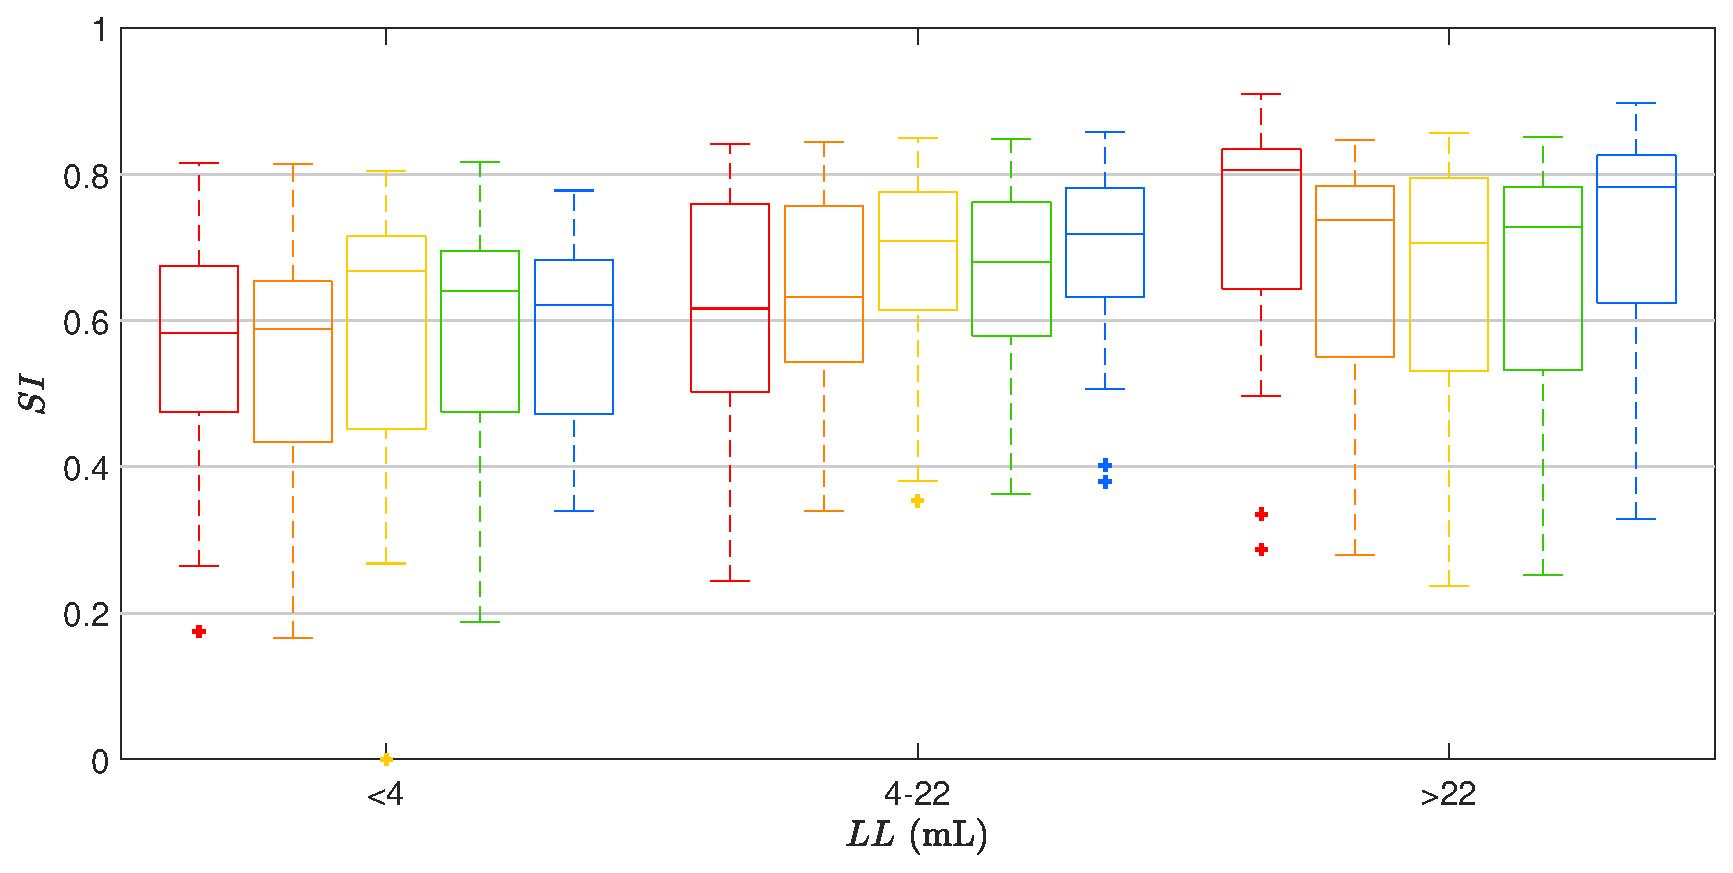
\includegraphics[scale=0.4]{ystd-box-si}
    \caption{$SI$}
  \end{subfigure}
  \\[0.5em]
  \begin{subfigure}{0.9\textwidth}
    \centering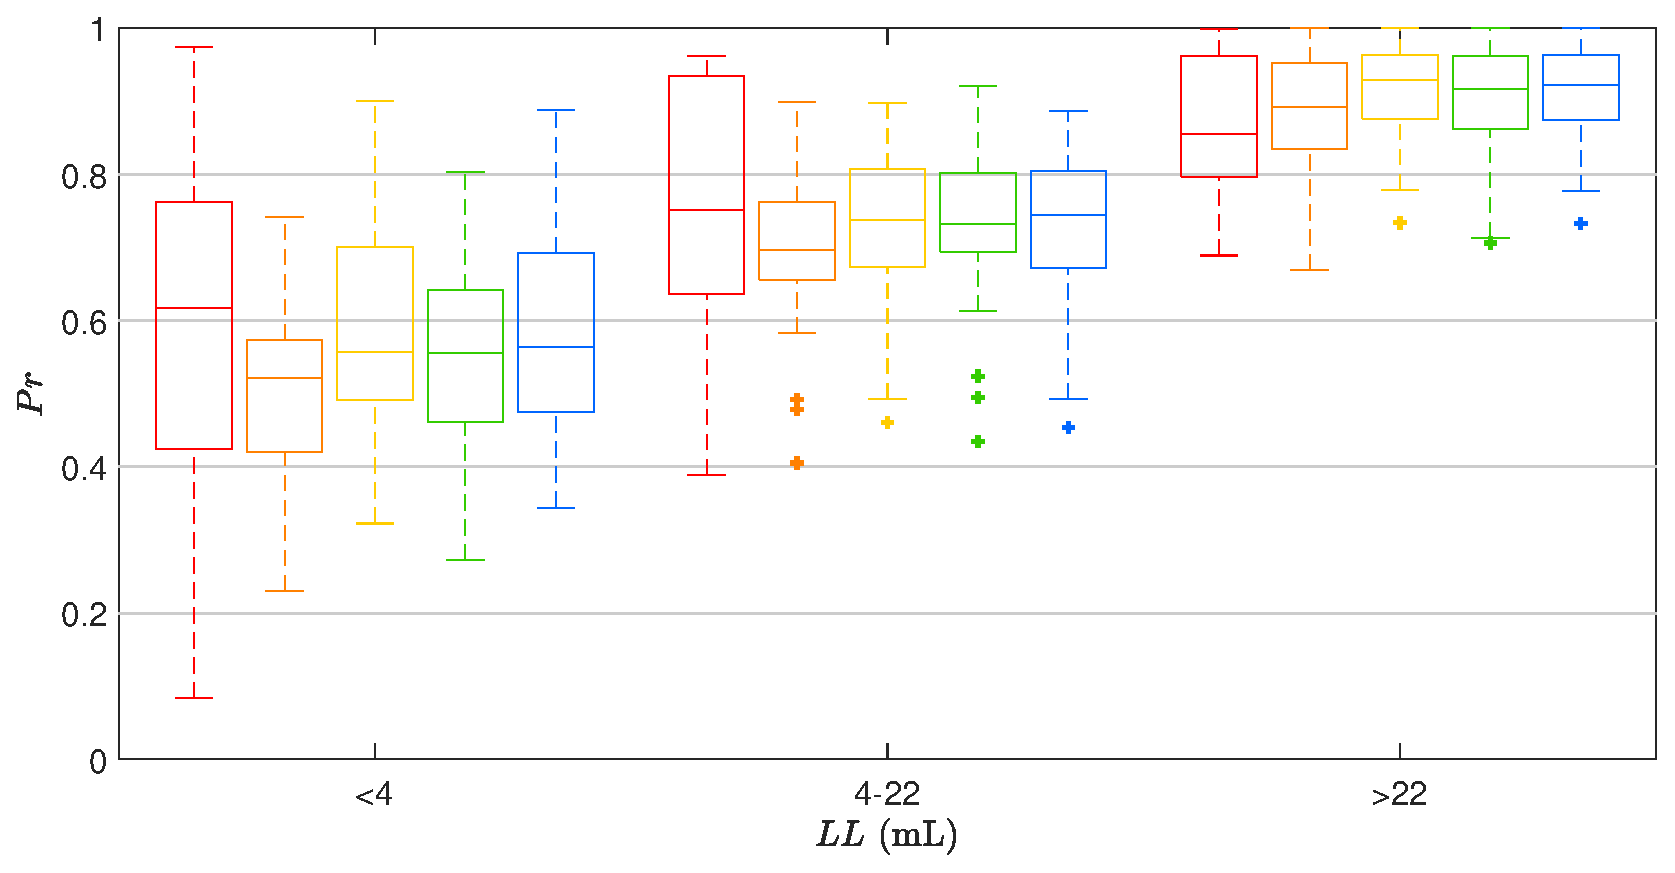
\includegraphics[scale=0.4]{ystd-box-pr}
    \caption{$Pr$} % chktex 35
  \end{subfigure}
  \\[0.5em]
  \begin{subfigure}{0.9\textwidth}
    \centering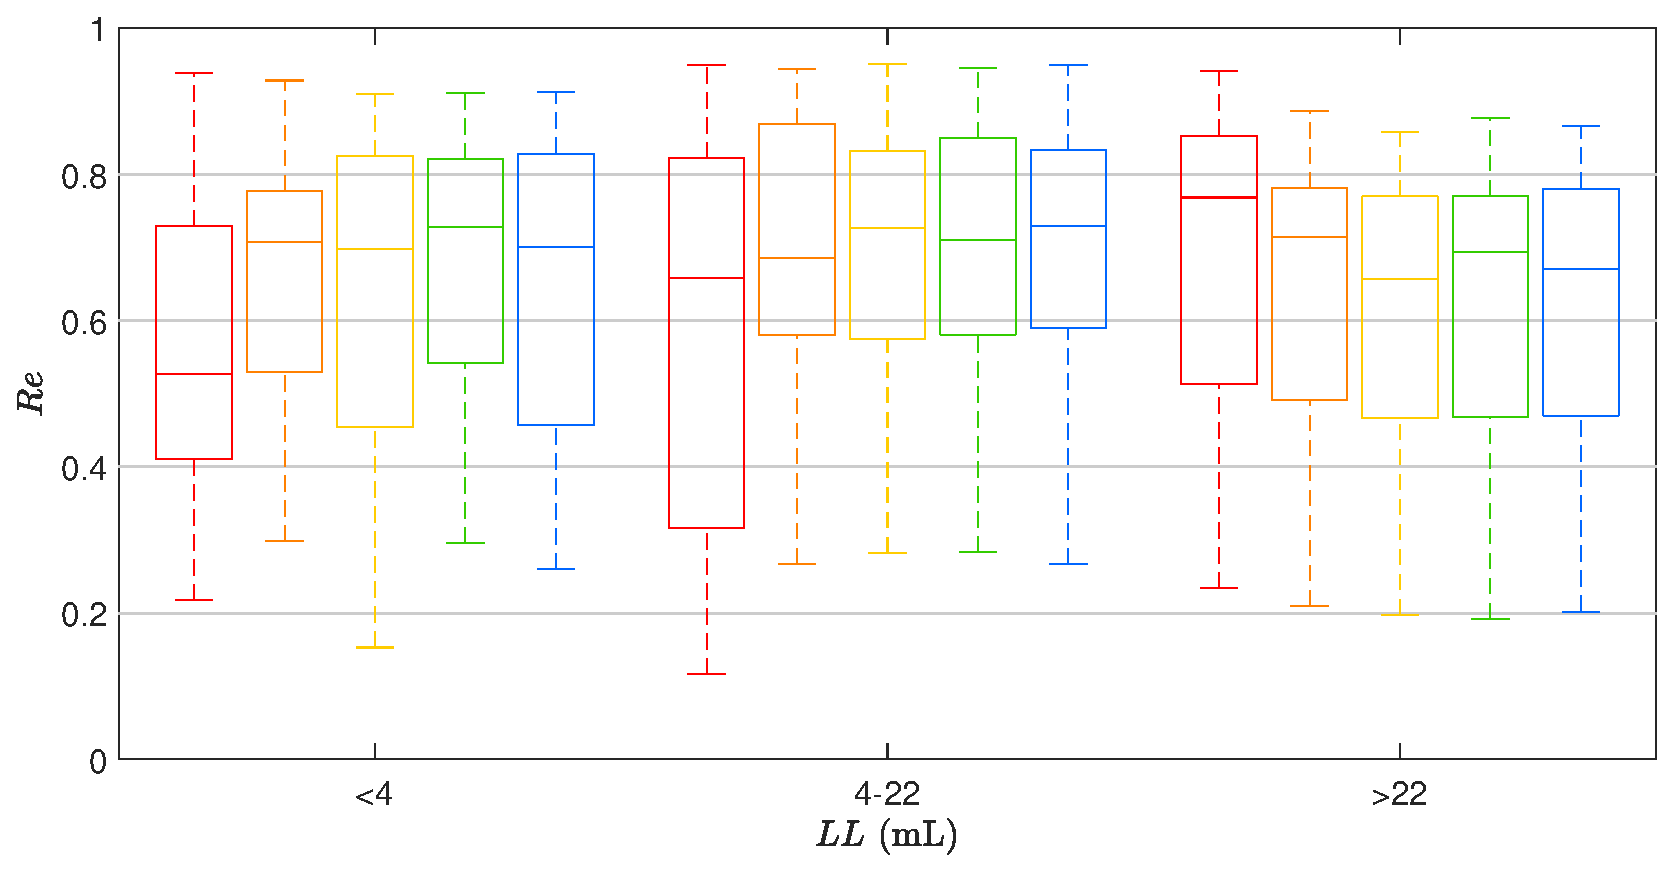
\includegraphics[scale=0.4]{ystd-box-re}
    \caption{$Re$}
  \end{subfigure}
  \caption{Comparison of the optimized model
    employing each graylevel standardization technique.}%
  \label{fig:seg-box-ystd}
\end{figure}
These results can be rationalized using Figure~\ref{fig:ystd-y},
where differences in image contrast produce predictable trade-offs between $Pr$ and $Re$. % chktex 35
For example, while histogram equalization (\textbf{HE}) gives good lesion contrast,
a large number of false positives are also typically incurred in the GM,
decreasing Precision.
Conversely, the optimal \textbf{HM3} method maintains good lesion contrast,
while minimizing GM/WM contrast.
% ==================================================================================================
\subsection{Regularization}\label{ss:exp-reg}
In this section, each of the regularization strategies
presented in Chapter~\ref{ch-pre} are explored,
particularly with respect to their impact on segmentation performance.
These include:
\begin{itemize}[itemsep=0pt,topsep=0pt]
  \item Pseudo-lesion regularization: $V$ -- number to include
  \item Parameter norm penalties: $\lambda$
  \item Data augmentation:
    $\mathrm{a}_{\textsc{r}}$ -- reflection;
    $\mathrm{a}_{\textsc{s}}$ -- shift.
\end{itemize}
Parameter image smoothing is further explored in~\ref{ss:exp-beta},
though optimization of both components is a chicken-and-egg problem,
since good regularizations are necessary to produce plausible parameter images
(cf.~obvious artifacts in Figure~\ref{fig:beta-base}),
while parameter image smoothing is similarly important.
Therefore, unless otherwise specified,
the default non-baseline parameter image smoothing: $G_{\sigma2}$ was used throughout this section.
\par
In order to characterize the contributions of each regularization technique independently,
each was added, one-at-a-time, to the baseline model.
This investigation did not use parameter image smoothing.
The performance metrics under each condition are summarized in Figure~\ref{fig:seg-box-ovb}.
\par
\begin{figure}
  \centering
  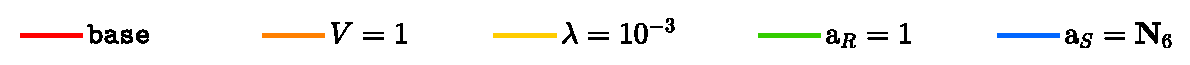
\includegraphics[scale=0.4]{ovb-box-leg}\\[0.5em]
  \begin{subfigure}{0.32\textwidth}
    \centering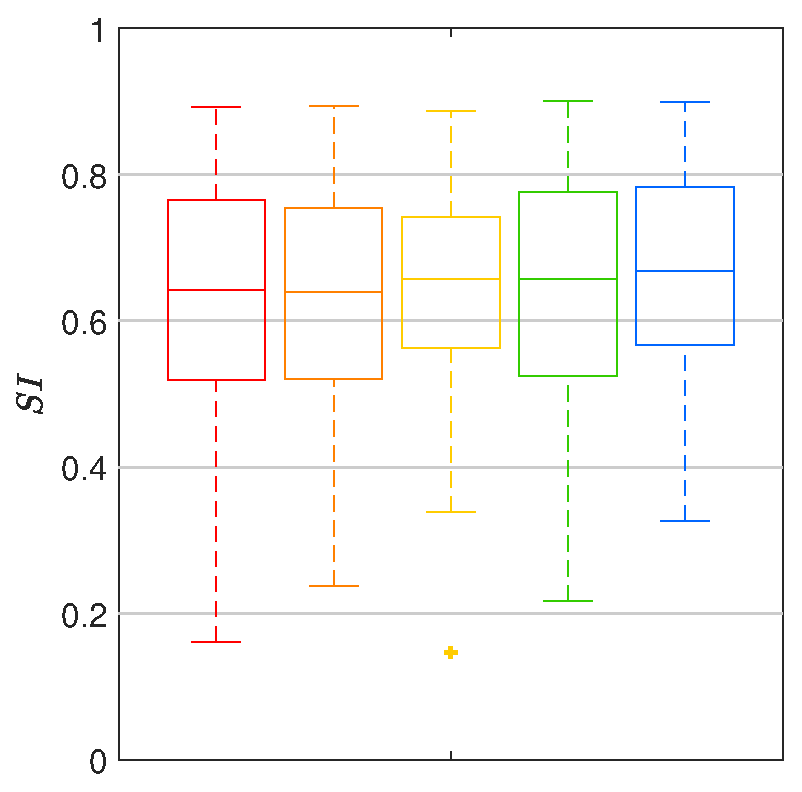
\includegraphics[scale=0.4]{ovb-box-si}
    \caption{$SI$}%
    \label{fig:seg-box-ovb-si}
  \end{subfigure}
  \begin{subfigure}{0.32\textwidth}
    \centering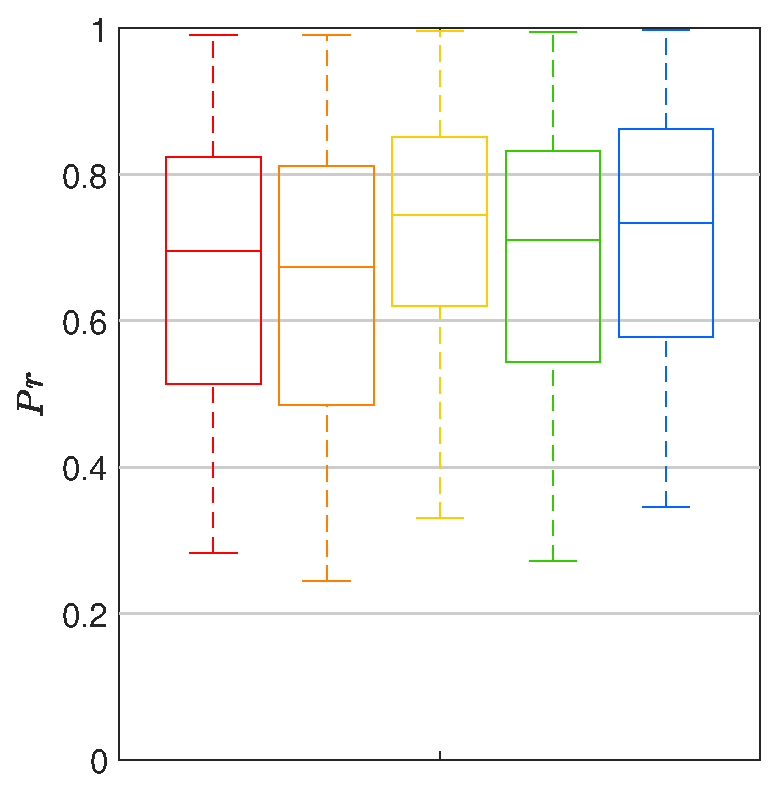
\includegraphics[scale=0.4]{ovb-box-pr}
    \caption{$Pr$}% % chktex 35
    \label{fig:seg-box-ovb-pr}
  \end{subfigure}
  \begin{subfigure}{0.32\textwidth}
    \centering\includegraphics[scale=0.4]{ovb-box-re}
    \caption{$Re$}%
    \label{fig:seg-box-ovb-re}
  \end{subfigure}
  \caption{Comparison of the baseline model under LOSO-CV
    incorporating each of the regularization strategies in isolation.}%
  \label{fig:seg-box-ovb}
\end{figure}
Each of the regularization techniques yielded
improvements in overall performance, as measured by Similarity Index.
However, as conjectured in~\ref{ss:vlr-reg-aug},
data augmentation strategies were most successful in boosting performance,
especially the shift augmentation.
Recall was most improved (fewer FN) through inclusion of pseudo-lesions; this is as expected,
since the no-lesion training voxels illustrated in Figure~\ref{fig:chmle-noles}
maintain the ability to predict $\hat{c} > 0$ under this condition.
This improvement came at the expense of a slight decrease in Precision.
Conversely, Precision was greatly improved through parameter norm penalties,
with an associated decrease in Recall.
This implies that overfitting associated with MLE estimation
most often results in False Positives,
which are minimized through the use of $\lambda$.
\par
The results in \S~\ref{ss:exp-toy-psu} demonstrated that use of additional
pseudo lesions did not have appreciable impacts on the fitted parameters
(cf. Figure~\ref{fig:toy-psu}), so additional selections of $V$ are not presented here.
Similarly, the reflection data augmentation is always helpful to include,
but no further investigations are needed.
Additional spatial data augmentations were similarly omitted for exploration,
since neighbourhoods larger than $\mathrm{N}_6$ (shifts larger than 1 voxel)
become less plausible as training images with small registration errors.
Therefore, only the $\lambda$ parameter was subject to further formal investigation
in terms of segmentation performance.
% --------------------------------------------------------------------------------------------------
\subsubsection{Parameter Norm Penalties}\label{sss:exp-lam}
Selection of the appropriate $\lambda$ was already partially explored in \S~\ref{ss:exp-toy-lam},
where it was determined that $\lambda \in [{10}^{-3},{10}^{-2}]$ provided a good trade-off
between limiting the magnitude of $\bb$ and maintaining MLE characteristics.
A similar range of $\lambda$ was explored in the full model: $[{10}^{-5},{10}^{-1}]$.
Exploration of the full model for each selection this time
employed the final optimized model parameters summarized in Table~\ref{tab:hyp-final},
in order to consider interactions between the different regularization strategies.
Performance metric results are again summarized using box plots in Figure~\ref{fig:seg-box-lam}.
\par
\begin{figure}
  \centering
  \includegraphics[scale=0.4]{lam-box-leg}\\[0.5em]
  \begin{subfigure}{0.32\textwidth}
    \centering\includegraphics[scale=0.4]{lam-box-si}
    \caption{$SI$}%
    \label{fig:seg-box-lam-si}
  \end{subfigure}
  \begin{subfigure}{0.32\textwidth}
    \centering\includegraphics[scale=0.4]{lam-box-pr}
    \caption{$Pr$}% % chktex 35
    \label{fig:seg-box-lam-pr}
  \end{subfigure}
  \begin{subfigure}{0.32\textwidth}
    \centering\includegraphics[scale=0.4]{lam-box-re}
    \caption{$Re$}%
    \label{fig:seg-box-lam-re}
  \end{subfigure}
  \caption{Comparison of the optimized model under LOSO-CV
    using different prior strengths $\lambda$.}%
  \label{fig:seg-box-lam}
\end{figure}
From these results, it can be seen that overal $SI$ performance
is surprisingly robust to the definition of $\lambda$.
This may be attributable to the effects of other regularizations,
especially the data augmentations and parameter image smoothing.
However, a maximum in Recall is achieved using $\lambda = 10^{-3}$.
This is desirable, since balancing $Pr$ and $Re$ should give % chktex 35
more accurate total LL estimates, and Recall is often much lower than Precision.
Therefore, $\lambda = 10^{-3}$ was selected as the optimal value.
% ==================================================================================================
\subsection{Parameter Images}\label{ss:exp-beta}
Noting the obvious artifacts in Figure~\ref{fig:beta-base},
generation of more plausible parameter images was a priority.
This section explores additional filtering operations applied to the
MAP estimated parameter images, whose aim was to both
improve the segmentation performance
and improve the qualitative plausibility of the resulting parameter images.
% --------------------------------------------------------------------------------------------------
\subsubsection{Smoothing}\label{sss:exp-beta-smooth}
The regularizations described in \S~\ref{ss:exp-reg} were surprisingly effective
at achieving these objectives, yielding the raw fitted parameter image
shown in the left most column of Figure~\ref{fig:beta-smooth}.
However, several artifacts are visible, including
voxels with very high magnitude in the sensitivity image $\mathcal{S}(x)$,
and large discontinuities between the voxels which
do and do not observe lesion examples during training in the threshold image $\mathcal{T}(x)$.
Therefore, the smoothing filters proposed in Table~\ref{tab:filters}
were each applied to the fitted parameter images in an attempt to correct these problems,
yielding the remaining panels in Figure~\ref{fig:beta-smooth}.
\par
\begin{figure}
  \centering
  \begin{tabu} to 4.7\sliceheight {X[c]X[c]X[c]X[c]X[c]X[c]} % chktex 1
    $(\cdot)$ & $\medfilt{3}$ & $\medfilt{5}$ & $G_{\sigma1}$ & $G_{\sigma2}$ & $G_{\sigma3}$
  \end{tabu}%
  \hphantom{\includegraphics[height=0.9\sliceheight]{cmap-beta-1}}\\[0.5em]
  \subfigureoverl[white]{$\mathcal{T}(x)$}{}{%
    \foreach \i in {1,2,3,4,5,6}{% % chktex 1
      \includegraphics[height=0.9\sliceheight]{T-\i.png}~}%
    \includegraphics[height=0.9\sliceheight]{cmap-beta-1}}
  \\[0.5em]
  \subfigureoverl[white]{$\mathcal{S}(x)$}{}{%
    \foreach \i in {1,2,3,4,5,6}{% % chktex 1
      \includegraphics[height=0.9\sliceheight]{S-\i.png}~}%
    \includegraphics[height=0.9\sliceheight]{cmap-beta-2}}
  \caption{Parameter images following different smoothing filters. Best viewed in colour.}%
  \label{fig:beta-smooth}
\end{figure}
Performance differences among the different filters
(Figure~\ref{fig:seg-box-beta}) were not large in magnitude.
However, the Gaussian filter with $\sigma = 2$ MNI voxels (3 mm)
achieved statistically higher performance than all other conditions except $G_{\sigma1}$.
This method also has the advantage of producing exceedingly smooth parameter images,
which are less likely to contain artifacts associated with the training set.
This advantage is contrasted with many other image filtering tasks in medicine,
where maintenance of image edges or other details is often a priority.
\par
Considering this result, one additional modification was made
to the model estimation procedure.
These details are presented in \S~\ref{ss:halfres}.
\begin{figure}
  \centering
  \includegraphics[scale=0.4]{beta-box-leg}\\[0.5em]
  \begin{subfigure}{0.32\textwidth}
    \centering\includegraphics[scale=0.4]{beta-box-si}
    \caption{$SI$}%
    \label{fig:seg-box-beta-si}
  \end{subfigure}
  \begin{subfigure}{0.32\textwidth}
    \centering\includegraphics[scale=0.4]{beta-box-pr}
    \caption{$Pr$}% % chktex 35
    \label{fig:seg-box-beta-pr}
  \end{subfigure}
  \begin{subfigure}{0.32\textwidth}
    \centering\includegraphics[scale=0.4]{beta-box-re}
    \caption{$Re$}%
    \label{fig:seg-box-beta-re}
  \end{subfigure}
  \caption{Comparison of the optimized model under LOSO-CV
    using different $\bb(x)$ smoothing.}%
  \label{fig:seg-box-beta}
\end{figure}
%\begin{table}
%  \centering
%  \caption{Image filters investigated for smoothing the estimated parameter images.}%
%  \label{tab:exp-filters}
%  \begin{tabular}{l}
%    \toprule
%    Name          \\ \midrule
%    $\medfilt{3}$ \\
%    $\medfilt{5}$ \\
%    $G_{\sigma1}$ \\
%    $G_{\sigma2}$ \\
%    $G_{\sigma3}$ \\
%    $\mathrm{Bilat}_{\sigma_y}^{\sigma_x}$ \\ \bottomrule
%  \end{tabular}
%\end{table}
% --------------------------------------------------------------------------------------------------
\subsubsection{Interpretation}\label{sss:exp-beta-interp}
The final parameter images provide concise descriptions of the VLR model.
The threshold image $\mathcal{T}(x)$ indicates the graylevels
corresponding to a 50\% probability of the lesion class $\hat{c}$,
while the sensitivity image $\mathcal{S}(x)$ describes
the rate of change in predicted probability near the threshold.
The regions of low threshold appear to align with
the typical distribution of lesions (cf. Figure~\ref{fig:mean-wmh}),
permitting even small hyperintensities in these areas to be recognized as WMH.
Conversely, lower threshold values are observed throughout the GM,
and in areas of common false positives, facilitating their exclusion.
The sensitivity image reflects the confidence of the model in the current prediction,
and is often lower in regions of TP and FP overlap.
For example, the border of the ventricles may contain hyperintensities
due to WMH or flow through artifacts in dilated ventricles,
and similarly, the corpus callosum is often bright,
but inconsistently included by manual raters in the WMH segmentation.
\par
Note that $\mathcal{S}(x)$ is significantly less important for segmentation performance.
One investigation which replaced this parameter image with its mean value
saw only a 0.24 decrease in median $SI$.
In fact, this approach mirrors the model proposed by~\citeauthor{Schmidt2017} in the LPA algorithm,
since only the $\b^0$ term is parameterized spatially.
This partly validates the modelling decisions by~\citeauthor{Schmidt2017},
though the advantages in estimability and performance
afforded by the current approach are significant.
% --------------------------------------------------------------------------------------------------
\subsubsection{Comparison with LPA Spatial Effect Parameter}\label{sss:exp-beta-lpa}
The inspiration for the current algorithm came from the LPA algorithm by~\citeauthor{Schmidt2017}.
In this method, the logistic regression is parametrized by only one spatial effect term: $\b^0(x)$.
This parameter was extracted from the toolbox%
\footnote{\texttt{sp\_mni2\_Bf2} in the \texttt{LST\_lpa\_stuff.mat} datafile from the toolbox.}
and reconstructed in MNI space, for comparison with the equivalent VLR-fitted parameter image.%
\footnote{The seven VLR model $\b^0(x)$ images from LOSO-CV folds
  using \textbf{SS} standardization were averaged,
  since this most closely approximates the standardization employed by the LPA algorithm.}
In order to facilitate visual comparison, the image means and variances were matched,
yielding the results shown in Figure~\ref{fig:beta-lpa}.
\par
\begin{figure}
  \centering
  \subfigureoverl[white]{LPA}{}{%
    \includegraphics[height=\sliceheight]{b0-LPA.png}
    \includegraphics[height=\sliceheight]{cmap-LPA}
  }\\[0.5em]
  \subfigureoverl[white]{VLR}{}{%
    \includegraphics[height=\sliceheight]{b0-VLR.png}
    \includegraphics[height=\sliceheight]{cmap-LPA}
  }
  \caption{Spatial effect intercept parameter images $\b^0(x)$ from the LPA and VLR algorithms.
    For visual comparison, image means and variances are matched. Best viewed in colour.}%
  \label{fig:beta-lpa}
\end{figure}
The two parameter images appear overall similar,
with areas of larger magnitude reflecting the usual distribution of lesions,
as in the regions of lower threshold in $\mathcal{T}(x)$.
The LPA parameter image is less detailed in most aspects,
but occasionally contains sharp artifacts from the estimation procedure,
which employs random sampling of spatial locations.
The VLR parameter image is more detailed, perhaps due to weaker assumptions about smoothness,
despite significant image filtering.
\par
Another notable difference is that the VLR $\b^0(x)$ is decreased in regions of the typical GM,
particularly in the insula and the along the mid-line, while the LPA image is not.
This is because the LPA model uses SPM-estimated GM and WM tissue segmentations
to apply tissue-specific graylevel standardization (type \textbf{SS}), and therefore assumes that
all standardized graylevels in the image are derived from a single normal distribution.
This approach was avoided in the VLR implementation,
since the SPM tissue segmentation almost always misclassifies WMH as GM,
resulting in erroneous standardization which decreases WMH contrast.
WMH contrast decreases because both the mean and variance
of the GM class are typically larger than that of the WM class;
subtracting the larger mean and dividing by the larger standard deviation
yields decreased WMH graylevels.
%%%%%%%%%%%%%%%%%%%%%%%%%%%%%%%%%%%%%%%%%%%%%%%%%%%%%%%%%%%%%%%%%%%%%%%%%%%%%%%%%%%%%%%%%%%%%%%%%%%%
\section{Optimized Model Summary}\label{ss:hyp-final}
Considering all experimental results, the optimal model hyperparameters were selected.
These values are summarized in Table~\ref{tab:hyp-final}.
Fitted parameter images from one LOSO-CV fold are also shown in Figure~\ref{fig:beta-final},
and an example segmentation is shown in Figure~\ref{fig:exseg}.
\par
\begin{table}
  \centering
  \caption{Model hyperparameters and optimized values.}%
  \label{tab:hyp-final}
  \begin{tabular}{llccc}
  	\toprule
  	Stage                            & Parameter            &         Notation          &            Type            &                Default                 \\ \midrule
  	\multirow{4}{*}{Pre-Processing}  & Reflect Augmentation & $\mathrm{a}_{\textsc{r}}$ &        $\mathbb{B}$        &                \true{}                 \\
  	                                 & Shift Augmentation   & $\mathrm{a}_{\textsc{s}}$ &       $\mathbf{N}_p$       &             $\mathbf{N}_6$             \\
  	                                 & Graylevel Transform  &        $\uptau_y$         &     $f: \Re\mapsto\Re$     &        $\uptau_{\textbf{RM3}}$         \\
  	                                 & Transform Mask       &       $\X_{\uptau}$       &      $\mathbb{B}(x)$       &          $\X_{\text{brain}}$           \\ \midrule
  	\multirow{7}{*}{VLR Fitting}     & Iterations           &            $T$            &        $\mathbb{Z}$        &                  $30$                  \\
  	                                 & Initial $\bb$        &        $\bb^{(0)}$        &          $\Re^2$           &                $[0,0]$                 \\
  	                                 & Estimation Scale     &       $\mathrm{r}$        &           $\Re$            &                 $0.5$                  \\
  	                                 & Learning Rate        &         $\alpha$          &           $\Re$            &                  $1$                   \\
  	                                 & Regularization       &         $\lambda$         &           $\Re$            &           $1\times{10}^{-3}$           \\
  	                                 & Pseudo-Lesions       &         $\bV(x)$          &    $\{\et\cdot\in\Re\}$    &             $\{y_{\max}\}$             \\
  	                                 & $\bb$ Filter         &         $F_{\bb}$         & $f: \Re(x) \mapsto \Re(x)$ & $\tilde{\bb}(x) = G_{\sigma2}(\bb(x))$ \\ \midrule
  	\multirow{1}{*}{Post-Processing} & Min Lesion  Size     &  $\mathrm{x}_{\min}^{c}$  &  $\Re\en(\text{mm}^{3})$   &                  $1$                   \\ \bottomrule
  \end{tabular}
  \tablepost{Notation.
    $\mathbb{B}$: boolean value;
    $\mathbb{Z}$: integer value;
    $\Re$: real value;
    $\Re^n$: vector;
    $\Re(x)$: image;
    $\mathbf{N}_p$: nearest $p$ voxel neighbourhood.}
\end{table}
\begin{figure}
  \centering
  \subfigureoverl[white]{$\mathcal{T}(x)$}{}{%
    \includegraphics[height=\sliceheight]{final-T.png}
    \includegraphics[height=\sliceheight]{final-cmap-T}}\\[0.5em]
  \subfigureoverl[white]{$\mathcal{S}(x)$}{}{%
    \includegraphics[height=\sliceheight]{final-S.png}
    \includegraphics[height=\sliceheight]{final-cmap-S}}
  \caption{Fitted parameter images $\mathcal{T}(x)$ and $\mathcal{S}(x)$
    from the first LOSO-CV fold of the final model. Best viewed in colour.}%
  \label{fig:beta-final}
\end{figure}
\begin{figure}
  \centering
  \foreach \i/\cap in {% % chktex 1
    I/$\mathrm{Y}(x)$,
    J/$\tilde{\mathrm{Y}}(x)$,
    T/$\mathrm{T}(x)$,
    S/$\mathrm{S}(x)$,
    Q/$\hat{\mathrm{C}}(x)$,
    P/$\et\cdot\et(x)$}{%
    \begin{subfigure}{0.15\textwidth}
      \centering\includegraphics[height=\sliceheight]{exseg-\i.png}
      \caption{\cap}
    \end{subfigure}~}
  \caption{Example segmentation. Best viewed in colour.}%
  \label{fig:exseg}
\end{figure}
% ==================================================================================================
\subsection{Segmentation Performance}\label{ss:exp-finalseg}
This section explores more detailed segmentation performance results
associated with the final model definition.
Median overall $SI$ performance was 0.69, a reasonable improvement over the baseline of 0.63,
and only 0.02 lower than the maximum possible performance of 0.71 using no cross validation.
As with the baseline model, results are broken down by scanner in Table~\ref{tab:seg-final},
where it can be seen that data from ISBI 2015 and MS 2016 (2)
have been the major beneficiaries of model improvements.
The same overall trends in scanner performance persist, however,
likely due to representation imbalances,
since there are only 5 images from each of the three MS 2016 scanners.
The model is also still significantly more precise than sensitive,
particularly for high LL, as shown in
Figures~\ref{fig:seg-final-pr}~and~\ref{fig:seg-final-scat-pr}.
Several subjects even reach near 100\% Precision.
Conversely, no overall improvements in Recall
were made during model optimization ($Re = 0.63$ again),
and Recall performance even decreases for high LL.
This is likely attributable to the histogram matching operation,
which begins to attenuate the WMH in images with high LL,
due to an implicit assumption that a consistent volume of hyperintensities will
appear in the image.
\par
\begin{table}
  \centering
  \caption{Final model performance metrics (median)}%
  \label{tab:seg-final}
  \input{figs/seg/final-performance}
\end{table}
\begin{figure}
  \centering
  \begin{subfigure}{0.32\textwidth}
    \centering
    \includegraphics[width=\textwidth]{final-box-si}
    \caption{Similarity Index (SI)}%
    \label{fig:seg-final-si}
  \end{subfigure}
  \begin{subfigure}{0.32\textwidth}
    \centering
    \includegraphics[width=\textwidth]{final-box-pr}
    \caption{Precision (Pr)}%
    \label{fig:seg-final-pr}
  \end{subfigure}
  \begin{subfigure}{0.32\textwidth}
    \centering
    \includegraphics[width=\textwidth]{final-box-re}
    \caption{Recall (Re)}%
    \label{fig:seg-final-re}
  \end{subfigure}
  \caption{Final model performance, stratified by LL tertiles.}%
  \label{fig:seg-final}
\end{figure}
\begin{figure}
  \centering
  \begin{subfigure}{0.32\textwidth}
    \centering
    \includegraphics[width=\textwidth]{final-scat-si}
    \caption{Similarity Index (SI)}%
    \label{fig:seg-final-scat-si}
  \end{subfigure}
  \begin{subfigure}{0.32\textwidth}
    \centering
    \includegraphics[width=\textwidth]{final-scat-pr}
    \caption{Precision (Pr)}%
    \label{fig:seg-final-scat-pr}
  \end{subfigure}
  \begin{subfigure}{0.32\textwidth}
    \centering
    \includegraphics[width=\textwidth]{final-scat-re}
    \caption{Recall (Re)}%
    \label{fig:seg-final-scat-re}
  \end{subfigure}
  \caption{Scatter plot of final model performance, with 3\ss{rd} order trend line
    and 90\% confidence interval shown in grey. Best viewed in colour.}%
  \label{fig:seg-final-scat}
\end{figure}
It is worth drawing attention to one consistent outlier from the WMH 2017 (1) scanner,
for which no TP were predicted (resulting in zero for all metrics).
The cause of this error was imperfect registration to MNI space by SPM,
resulting in bright skull tissue within the static brain mask.
While this did not yield any FP, due to the ability of the VLR model to exclude these regions,
the large number of other hyperintensities in the image
affected the histogram matching operation used for standardization,
resulting in WMH which were much darker than usual, as noted above.
\par
Figure~\ref{fig:ba-final} shows the volume agreement between
the manually segmented WMH and the VLR-estimated WMH.
As predicted by the $Pr$ and $Re$ results, % chktex 35
the model tends to underestimate the LL,
with underestimation getting worse for very high LL.
This trend is likely a result of the histogram-matching graylevel standardization,
since this histogram-based nonlinear transformation,
acts to equalize the proportion of hyperintensity in every image.
Therefore, in subjects with more hyperintensities, lesion contrast is reduced.
This unfortunately led to a poor overall volume agreement, as measured by ICC: 0.58.
\par
\begin{figure}
  \centering
  \includegraphics[width=0.8\plotwidth]{final-ba-1}
  \includegraphics[width=0.8\plotwidth]{final-ba-2}
  \caption{Bland-Altman plot showing total LL agreement between manual and VLR-segmented WMH.
    Shown in Log-scale to better illustrate results for small LL.}%
  \label{fig:ba-final}
\end{figure}
Finally, reflecting on the original motivations for including spatial features in the model
(cf. Figure~\ref{fig:tpfpfn-thropt} in \S~\ref{sss:limits-flair}),
the distributions of TP, FP and FN from the LOSO-CV segmentations of the VLR model
are presented again here in Figure~\ref{fig:tpfpfn-final}.
The distribution of FP is now limited to the same spatial regions as TP,
implying that practically all the problematic regions of FP shown in Figure~\ref{fig:tpfpfn-thropt}
have been managed though the spatial parametrization.
In fact, the distributions of FP and FN are now essentially identical,
suggesting that little more can be done with the current model to distinguish these classes.
This conclusion is also corroborated by the No-CV segmentation performance results,
which indicate a maximum possible performance of the current model.
Potential methods of augmenting the model to solve this problem
will be explored in the next chapter.
\begin{figure}
  \centering
  \foreach \i in {TP,FP,FN}{% % chktex 1
    \subfigureoverl[white]{$\i(x)$}{}{%
      \includegraphics[height=\sliceheight]{final-\i.png}
      \includegraphics[height=\sliceheight]{final-cmap-tri}}\\[0.5em]}
  \caption{Distribution of True Positives (TP), False Positives (FP), and False Negatives (FN)
    from all LOSO-CV folds of the final model. Best viewed in colour.}%
  \label{fig:tpfpfn-final}
\end{figure}
% --------------------------------------------------------------------------------------------------
\subsubsection{``Turing Test''}\label{sss:exp-turing}
In order to determine whether the VLR algorithm produces results which are indistinguishable
from other human raters, it was first necessary to establish a measure of human performance.
To do so, the inter-rater agreement was calculated for those datasets
having multiple manual segmentations: MS 2016~\cite{MSSEG2016} and ISBI 2015~\cite{MSISBI2015}.
Since $SI$ is a true metric,
the direction of comparison (test-to-standard or standard-to-test) does not matter.
Therefore, the $SI$ can be computed between any two human raters.
\par
The inter-rater $SI$ was calculated in all possible pair-wise comparisons among the 7 raters
(7-choose-2 = 21 total), then averaged, for all 15 available images in the MS 2016 dataset.
The same procedure was repeated for the two raters, for all 21 images in the ISBI 2015 dataset.
The ICC (cf. \S~\ref{ss:exp-metrics}) between segmented lesion volumes was also calculated.
These results, summarized Table~\ref{tab:interrater-inhouse},
are consistent with other reports in the literature (Table~\ref{tab:interrater-cite}).
\par
\begin{table}
  \centering
  \caption{Mean inter-rater agreement measures
    for manual WMH segmentation calculated for the available data.}%
  \label{tab:interrater-inhouse}
  \begin{tabular}{clcccc}
    \toprule
    Ref & Dataset & Raters & Data & SI & ICC \\
    \midrule
    \cite{MSSEG2016}  & MSSEG 2016   &  7  & 15 images & 0.63$\pm$0.16 & 0.91 \\ % chktex 2
    \cite{MSISBI2015} & MS 2015 ISBI &  2  & 21 images & 0.73$\pm$0.10 & 0.98 \\ % chktex 2
%    ---               & Dataset A    & --- & 96 images & 0.64$\pm$0.17 & 0.58 \\
    \bottomrule
  \end{tabular}
\end{table}
Next, non-parametric unpaired tests (\texttt{ranksum} in MATLAB) compared
the human inter-rater $SI$ values ($n=21$, $n=315$)
to the VLR-vs-human $SI$ values ($n=96$),
to test for significant differences.
Differences were significant in the MS 2015 ISBI comparison,
but not for MS 2016 comparison.
This implies that the VLR algorithm was indistinguishable from the human raters
in the MS 2016 dataset.
%%%%%%%%%%%%%%%%%%%%%%%%%%%%%%%%%%%%%%%%%%%%%%%%%%%%%%%%%%%%%%%%%%%%%%%%%%%%%%%%%%%%%%%%%%%%%%%%%%%%
\section{Comparison with Other Methods}
While the selection of freely available data for most of this work
permits direct replication of the validation conditions by future works,
several existing algorithms have already been deployed for use by other researchers.
It is therefore possible to compare the performance of these methods with
the proposed VLR model directly.
% ==================================================================================================
\subsection{Lesion Prediction Algorithm (LPA)}\label{ss:exp-lpa}
The LPA algorithm is the only freely available FLAIR-only WMH segmentation tool,
and has been used in several comparisons with other methods%
~\cite{Egger2017,Griffanti2016,Brosch2016}.%
\footnote{These methods cite~\cite{Schmidt2012},
  which is the reference requested for citations related to the LST toolbox.
  The PhD thesis describing the LPA algorithm was also only published in~\citeyear{Schmidt2017}.}
For this reason, the segmentation performance of the LPA algorithm
was compared to the proposed algorithm under LOSO-CV.
In order to binarize the probabilistic class images produced by the LPA algorithm,
a user-defined threshold can be used.
To reduce the bias of the comparison,
this threshold is optimized for each of the same LOSO-CV folds as for the VLR algorithm.
No other LPA parameters can be specified by the user.
\par
Box plots comparing the segmentation performance metrics, stratified by LL
are given in Figure~\ref{fig:seg-lpa}, and
the Sign Rank test was again used to test for significant differences.
The VLR algorithm easily outperforms its LPA forerunner
in $SI$ at small and medium LL ($p < 0.001$),
while differences at large LL were not significant.
Overall, median $SI$ were 0.69 and 0.58, respectively, also significantly different ($p < 0.001$).
The VLR algorithm was also more precise at all lesion loads than the LPA algorithm ($p \le 0.001$),
but overall had lower recall, mainly due to differences at high LL ($p < 0.001$).
\par
\begin{figure}
  \centering
  \includegraphics[scale=0.4]{lpa-box-leg}\\
  \begin{subfigure}{0.32\textwidth}
    \centering
    \includegraphics[width=\textwidth]{lpa-box-si}
    \caption{Similarity Index (SI)}%
    \label{fig:seg-lpa-si}
  \end{subfigure}
  \begin{subfigure}{0.32\textwidth}
    \centering
    \includegraphics[width=\textwidth]{lpa-box-pr}
    \caption{Precision (Pr)}%
    \label{fig:seg-lpa-pr}
  \end{subfigure}
  \begin{subfigure}{0.32\textwidth}
    \centering
    \includegraphics[width=\textwidth]{lpa-box-re}
    \caption{Recall (Re)}%
    \label{fig:seg-lpa-re}
  \end{subfigure}
  \caption{Comparison of VLR model performance versus LPA}%
  \label{fig:seg-lpa}
\end{figure}
These results might be explained by the parameter images shown in Figure~\ref{fig:beta-lpa}:
while the VLR algorithm learns to exclude potential FP in the GM by spatial location alone,
the LPA algorithm maintains sensitivity to hyperintensities in these areas.
As a result, the VLR algorithm is very precise, at the expense of sensitivity,
while the LPA algorithm is able to detect more peripheral lesions, sacrificing precision.
% ==================================================================================================
\subsection{2017 WMH Segmentation Challenge Results}\label{ss:exp-wmhseg17}
The proposed VLR method was submitted to the WMH Segmentation Challenge at MICCAI 2017.
The available training data included T1 and FLAIR MRI
from 60 subjects and 3 different scanners (20+20+20),
while the testing data comprised
110 total subjects from 5 different scanners (30+30+30+10+10).
A total of 20 teams participated,
and teams were scored using a combination of the following 5 performance metrics:
\begin{itemize}[itemsep=0pt,topsep=0pt]
  \item Similarity Index -- \texttt{dsc}
  \item Hausdorff distance (modified, 95\ss{th} percentile)~\cite{Dubuisson1994} -- \texttt{h95}
  \item Percent volume difference -- \texttt{avd}
  \item Recall for individual lesions -- \texttt{recall}
  \item Similarity Index for individual lesions -- \texttt{f1}
\end{itemize}
Scores for ``individual lesions''
count each set of connected ($\mathbf{N}_{26}$) voxels
-- i.e.\ one ``lesion'' -- as an single observation,
which can be classified as
TP if there is at least one voxel of overlap with the manual segmentation,
FP if a predicted lesion has no corresponding voxels in the manual segmentation, and
FN if a manual lesion has no corresponding voxels in the predicted lesion.
Each of the 5 metrics are averaged across all 110 test subjects,
and the overall score considers an average of all 5 metrics
after scaling by the range of minimum and maximum scores achieved by the 20 challengers;
this score is $\in [0,1]$ where lower is better.%
\footnote{For more information, see \hreftt{http://wmh.isi.uu.nl/evaluation/}.}
\par
The VLR method achieved an average SI performance of 0.70 on the test data,
which is actually slightly higher than the LOSO-CV predicted performance in \S~\ref{ss:hyp-final}.
Using the challenge metric scaling, this represents a relative score of 82.3\%,
ranking the VLR method 8\ss{th} in this dimension.
Other metrics did not look so favourably on the proposed method,
including lesion-wise recall (\texttt{recall} = 0.25), where VLR ranked dead last.
Considering these metrics in the overall ranking,
the VLR method ranked only 15\ss{th} of 20 teams, with a score of 0.4159.
The challenge performance report provided by the competition organizers
is given in Figure~\ref{fig:wmh-results}.%
\footnote{Detailed results and competitor methods descriptions are available at:
  \hreftt{http://wmh.isi.uu.nl/results/}.}
\par
\begin{sidewaysfigure}
    \centering
    \includegraphics[width=\textheight]{wmh-results.png}\\
    \caption{Results report for the submitted method provided by the WMH Segmentation Competition.}%
    \label{fig:wmh-results}
\end{sidewaysfigure}
At the MICCAI 2016 MSSEG Competition, only 4 of the 15 submitted methods used deep learning,
while the 2017 competition saw 15 of 20 methods use this approach,
\textit{including the top performing 13 methods}.
This impressive and sudden display of model dominance should not be taken for granted,
especially considering the large number of previously proposed non-deep WMH segmentation methods
(cf.~\S~\ref{ss:prior-proposed}).
The top performing non-deep method (team ``\texttt{tig}'' 14\ss{th} place, overall score of 0.3858)
uses an adaptation of the unsupervised unified mixture model described in~\cite{Sudre2015}.
This method outperforms the VLR submission in both lesion-wise metrics
(\texttt{recall} = 0.38 vs 0.25, and \texttt{f1} = 0.42 vs 0.35),
but performs worse in mean SI (0.60 vs 0.70), and additionally requires both T1 and FLAIR images.
\par
These results also highlight a major and perhaps flawed assumption used
throughout the current work:
that optimizing ``segmentation performance'' is equivalent to
maximizing the Similarity Index with manual segmentations.
In fact, diagnostic criteria considering WML often focus instead on
identification of new lesions in different spatial locations~\cite{Polman2011,Sorbi2012}.
Limitations such as this will be further discussed in the next chapter.
% --------------------------------------------------------------------------------------------------
% ==================================================================================================
%%%%%%%%%%%%%%%%%%%%%%%%%%%%%%%%%%%%%%%%%%%%%%%%%%%%%%%%%%%%%%%%%%%%%%%%%%%%%%%%%%%%%%%%%%%%%%%%%%%%

%Finally,  ... (cf.~Training / Validation / Test Sets in~\cite{Ripley1995})
